\documentclass[12pt,a4paper,oneside]{report}
\usepackage{indentfirst}
\usepackage{times}
\usepackage{array}
\usepackage{multirow}
\usepackage{ragged2e}
\setlength\parindent{1cm}
\renewcommand{\baselinestretch}{1.50}\normalsize
\usepackage{anysize}
\marginsize{1.25in}{.75in}{1in}{1in}
\usepackage{graphics}
\usepackage{graphicx}
\usepackage{epsfig}
\usepackage{booktabs}
\usepackage[fleqn]{amsmath}
\usepackage{amsfonts}
\usepackage{textcomp}
\usepackage{graphicx}
\usepackage{setspace}
\usepackage{fancyhdr}
\usepackage{truncate}
\usepackage{nomencl} 
\usepackage{acronym}
\usepackage{array}
\usepackage{float}
\usepackage{caption}
\usepackage{subfig}
\usepackage[overload]{textcase}
\usepackage{listings}
\renewcommand{\nomname}{List of Abbreviations}
\usepackage{makeidx}
\makeindex
\makenomenclature
\newcommand{\quotes}[1]{``#1''}
\usepackage{titlesec}
\titleformat{\chapter}[display]
{\normalfont\Large\bfseries\centering}
{\chaptertitlename\ \thechapter}{15pt}{\LARGE}
\titleformat{\section}{\large\bfseries}{\thesection}{1em}{}
\titleformat{\subsection}{\normalsize\bfseries}{\thesubsection}{1em}{}
\renewcommand{\chaptermark}[1]{\markboth{ \emph{#1}}{}}

\printnomenclature[5em]
\pagestyle{fancy}
%\headheight 1pt
	\renewcommand{\footrulewidth}{1.2pt}
\renewcommand{\headrulewidth}{1.2pt}
\rhead{\scriptsize {\leftmark}}

\lhead{\small{College of Engineering, Cherthala \;\;\;\;\;\;\;\;\;\;\;\;\;\;\;\;\;\;}}
\rfoot{\thepage}
\cfoot{\empty}
\lfoot{\small{Department of Computer Science \& Engineering}}
\renewcommand{\figurename}{Fig.}
\begin{document}
\renewcommand\bibname{References}
\begin{titlepage}
\begin{center}
\Large{\textbf{MAJOR PROJECT REPORT}}\\
\textbf{ON}\\
\vspace{.05 in}
\begin{singlespace}
\LARGE{\textbf{EBA - Electricity Board Application }}\\
\end{singlespace}
\vspace{.1 in}
\Large{\textit{Submitted By }}\\
\begin{singlespace}
\Large{\textit{\textbf{AJESH M (Reg. No. 12141201)}}} \\
\Large{\textit{\textbf{MUHAMMED NADIRSHA (Reg. No. 12143615)}}} \\
\Large{\textit{\textbf{RIBIN ROY (Reg. No. 12143620)}}} \\
\Large{\textit{\textbf{SREENIVAS S NAIK (Reg. No. 12143622)}}} \\
\end{singlespace}
\Large{\textit{\textit{under the guidance of}}}\\
\Large{\textit{Mrs. Anitha M. A.}}\\
\begin{singlespace}
\Large{\textit{(Assistant Professor)}}\\
\Large{\textit{Computer Science \& Engineering}}
\end{singlespace}
\vspace{.05in}
\begin{figure}[h]
\begin{center}

\epsfig{width=1.82 in, file=logo.jpg}
\end{center}
\end{figure}
\begin{singlespace}
\large{\textbf{MARCH 2017}}\\
\vspace{.1in}
\large{\textbf{DEPARTMENT OF COMPUTER SCIENCE AND ENGINEERING\\COLLEGE OF ENGINEERING,CHERTHALA\\ PALLIPPURAM P O, ALAPPUZHA-688541, \\PHONE: 0478 2553416, FAX: 0478 2552714\\http://www.cectl.ac.in}}
\end{singlespace}
\end{center}
\end{titlepage}

\begin{titlepage}
\begin{center}

\large{\textbf{MAJOR PROJECT REPORT}}\\
\begin{singlespace}
\LARGE{\textbf{EBA - Electricity Board Application }}\\
\end{singlespace}


\Large{\textit{Submitted By }}\\
\begin{singlespace}
\Large{\textit{\textbf{AJESH M (Reg. No. 12141201)}}} \\
\Large{\textit{\textbf{MUHAMMED NADIRSHA (Reg. No. 12143615)}}} \\
\Large{\textit{\textbf{RIBIN ROY (Reg. No. 12143620)}}} \\
\Large{\textit{\textbf{SREENIVAS S NAIK (Reg. No. 12143622)}}} \\
\end{singlespace}
\Large{\textit{\textit{under the guidance of}}}\\
\Large{\textit{Mrs. Anitha M. A.}}\\
\begin{singlespace}
\large{\textit{In partial fulfillment of the requirements for the award of the degree}\\
\large{ \textit{of}}\\
\large{\textit{Bachelor of Technology} }\\
\large{\textit{in}}\\
\large{\textit{Computer Science and Engineering}}\\
\large{\textit{of}}\\
\large{\textit{Cochin University Of Science And Technology }}}\\
\end{singlespace}
\begin{figure}[h]
\begin{center}

\epsfig{width=0.9in, file=logo.jpg}
\end{center}
\end{figure}
\begin{singlespace}

\Large{\textbf{MARCH 2017\\Department of Computer Science and Engineering\\College of Engineering, Pallippuram P O, Cherthala, Alappuzha Pin: 688541, \\Phone: 0478 2553416, Fax: 0478 2552714\\http://www.cectl.ac.in}}
\end{singlespace}
\end{center}
\end{titlepage}


\begin{titlepage}
\begin{center}

\large{\textbf{DEPARTMENT OF COMPUTER SCIENCE \& ENGINEERING}}\\
\large{\textbf{COLLEGE OF ENGINEERING CHERTHALA\\ALAPPUZHA-688541}}\\
\end{center}
\begin{figure}[h]
\begin{center}

\epsfig{width=1.7in, file=logo.jpg}
\end{center}
\end{figure}
\begin{center}
\large{\textbf{C E R T I F I C A T E}}\\
\end{center}
\begin{spacing}{1.5}
\begin{center}
\par\ This is to certify that, the Major Project Report submitted by \\
\end{center}
\raggedright Name \hspace{0.21in}: \hspace{0.21in}\hspace{3.4in}Date \hspace{0.1in}: \\
\raggedright Reg.No \hspace{0.10in}: \hspace{0.21in}\\
\centering \textbf{EBA-Electricity Board Application}\\
\justify
In partial fulfillment of the requirement of course of the Bachelor of Technology, (B. Tech) in Computer Science \& Engineering prescribed by Cochin University of Science \& Technology during the academic year 2016-2017.\\ 
\end{spacing}
\begin{tabbing}
xxxxxxxxxxxxxxxxxxxxxxxxxxxxxxxxxxxxxx\= xxxxxxxxxxxxxxxxxxxx\= \kill
\hspace{.4in}{\bf Guide} \>\hspace{-.5in}{\bf Co-ordinator}\hspace{1.7in}{\bf  HoD  } \\
\end{tabbing}
\begin{tabbing}
xxxxxxxxxxxxxxxxxxxxxxxxxxxxxxxxxxxxxx\= xxxxxxxxxxxxxxxxxx\= \kill
%\vspace{0.3in}\\
\hspace{.15in}{\bf{Mrs. Anitha M. A.}}   \>\hspace{-.7in}{\bf Mr. Muhammed Ilyas H} \hspace{.65 in}{\bf Dr. Preetha Theresa Joy }\\
\hspace{.15in}Assistant Professor    \>\hspace{-.7in}Assistant Professor\>\hspace{.23in}Professor\\
\hspace{.1in} Computer Science \& Engg    \>\hspace{-.75in}    Computer Science \& Engg \>\hspace{.18in}    Computer Science \& Engg\\

\end{tabbing}
\end{titlepage}

  \newpage
  \section*{\begin{center}\Large ACKNOWLEDGMENT\end{center}}
  \thispagestyle{empty}
  \par
  \hspace{0.1in}
 \par  I take this opportunity to express my sincere gratitude to the people who have been instrumental in the successful completion of my major project.\\
 \par  For every endeavor in my life, the help of the Lord has always followed. I have yet again experienced his loving kindness while preparing for this project. I would like to express my sincere thanks to the Principal, \textbf{Dr. Mini M. G} , for her valuable support and advice. I would also like to thank our Head Of Computer Science Department, \textbf{Dr. Preetha Theresa Joy} (Professor, Department of Computer Science) for her support. I express my heartfelt gratitude to my project coordinator, \textbf{Mr. Muhammed Ilyas H} (Assistant Professor, Department of Computer Science) for his valuable help and support. I would like to thank my project Guide,\textbf{ Mrs. Anitha M.A }(Assistant Professor, Department of Computer Science) for her support and guidance. I would also like to thank my project sub coordinator,\textbf{ Mrs. Sreelakshmi Murali }(Assistant Professor, Department of Computer Science) for her support and guidance.\\
 \par I am indebted to all teaching and non-teaching staff of the Department of Computer Science \& Engineering, friends and family for their co-operation and support, with out which I could never have completed the project this well.\\
 
 \newpage
 \section*{\begin{center}\Large ABSTRACT\end{center}}
 \thispagestyle{empty}
 \par
 \hspace{0.1in}
 \par Today in this digital world, people are fed up with the problems and delay in the functioning
 of Electricity Board. By the implementation of this application all the problems that
 are associated with the existing system will be reduced.
 In the Electricity Board Application there are number of features to help people to know
 about the information regarding time schedule for power cuts, last date for bill payment and
 previous meter reading histories facility to pay bill online, application for new connection, facility to register complaints and to check their current status. We know that the power cuts are more in the recent times and we are much irritated,
 though the information about these power cuts are published in the dailies, people wont spot
 the news efficiently, by using this application, people gets information about this data to their
 application installed on the phone. Consumers get notification about their pay date for the bill,
 until they have paid the bill. User even have the facility to know about their former bill
 payments. People can even pay the bill online through this application. Application also includes facility to register complaints about current connection and check its status through which consumer will get convenient response. People can also
 apply for a new connection through this application and thus avoiding too much offline steps.

\pagenumbering{roman}
\setcounter{page}{0} 
\tableofcontents

\listoffigures


\def\addsymbol #1: #2#3{\;\;\;\;\;\;\;\;\;\;\;\;\;\;\;\;\;\;\;\;\;\;\;$#1$ \> \;\;\;\;\;\;\;\;\;\;\;\;\;\;\;\;\;\;\;\;\;\;\;\;\;\; \parbox{5in}{#2}\\}



\renewcommand*\thesection{\thechapter.\arabic{section}}
\newpage
\pagestyle{fancy}
%\headheight 2pt
\renewcommand{\footrulewidth}{1.2pt}
\renewcommand{\headrulewidth}{1.2pt}
\rhead{\scriptsize {\leftmark}}
%\chead{Middle top}
\lhead{\small{College of Engineering, Cherthala \;\;\;\;\;\;\;\;\;\;\;\;\;\;\;\;\;\;}}
\rfoot{\thepage}
\cfoot{\empty}
\lfoot{\small{Department of Computer Science \& Engineering}}


\chapter{INTRODUCTION}
\label{intro}
\pagenumbering{arabic}
\setcounter{page}{1}
%\hspace{0.1in}
\section{PURPOSE}
\par 
This system reduces the complexities that are occur during the interaction with the Electricity
Board. We know that the power cuts are more in the recent times and we are much
irritated, though the information about these power cuts are published in the dailies, people
wont spot the news efficiently, by using this application, people gets information about this
data to their application installed on the phone. Consumers get notification about their pay date
for the bill, until they have paid the bill. Consumers even have the facility to know about their
former bill payments. Consumers can even pay the bill online through this application. People
can also apply for a new connection through this application and thus avoiding too much offline
steps.

\section{SCOPE}
\par Today, people are surfeited with the predicaments and procrastinations in the functioning
of Electricity Board. By the implementation of this application all the problems that are
associated with the existing system will be reduced. In the Electricity Board Application there
are number of features to help people to know about the information regarding time schedule
for power cuts, last date for bill payment and previous meter reading histories, facility to pay
bill online, online complaint registration, application for new connection etc. This proposed system will reduce the complexities that may occur during the consumer synergy with the Electricity Board.
The separate login for linemen will help in reducing the intricacies while assigning line man for a particular work in corresponding area.In addition to this, EBA users can apply for new electricity connection by dint of this Application.
Posterior, the user will be apprised with the requirement of soft copies of forms to be verified (if any) by the administrator in authority. With all these, the elucidation between consumers and electricity board will be acclaimed. \\
\chapter{SYSTEM ANALYSIS}

%\hspace{0.1in}

\section {EXISTING SYSTEM}
\par  In the existing system people are suffering a lot because of the irregularities while interacting
with the electricity board. By the implementation of this application all the problems
that are associated with the existing system will be reduced.

\subsection {Proposed System}
In the Proposed system there are number of features to help people to know about the
information regarding time schedule for power cuts, last date for bill payment and previous
meter reading histories, facility to pay bill Online, application for new connection.
%\newpage
\subsection {Product Functions}
The major functions of the product are:
\begin{itemize}
 \item Verified consumer accounts.
 \item Verified lineman accounts.
 \item Online Bill payment.
 \item Alert about the last date for the bill to be paid.
 \item Previous Bill payment details.
 \item Notification about power cuts.
 \item Apply for new connection.
 \item New connection status.
 \item Consumer complaints.
 \item Complaint status.
 
\item The output will be available in the form of both text and speech.
\end{itemize}

\section{LIFE CYCLE MODEL}
The paradigm chosen for this project is prototype life cycle model. Prototype model should be used when the desired system needs to have a lot of interaction with the end users. Prototype ensures that the end users constantly works with the system and provide a feedback which is incorporated in the prototype to result in a usable system. They are excellent for designing good human computer interface systems. For the entire graphical user interfacing prototype life cycle model is used. The basic idea here is that instead of freezing the requirements before a design or coding can proceed, a through way prototype is built to understand the requirements. By using this prototype, the client can get an ``actual feel" of the system, since the interactions with the prototype can enable the client to better understand the requirements of the desired system. Prototyping is an attractive idea for complicated and large systems for which there is no manual process or existing system to help determining the requirements. The prototype is usually not complete systems and many of the details are not built in the prototype. The goal is to provide a system with overall functionalities.
\par
Users are actively involved in the development. Since in this methodology a working model of the system is provided, the users get a better understanding of the system being developed. Errors can be detected much earlier. Quicker user feedback is available leading to better solutions. Missing functionality can be identified easily. Confusing or difficult functions can be identified. Required validation, quick implementation of, incomplete, but functional, application.
\par As a part of applying prototyping in our project, first we generated a rough interface of our Mahallu Management. Later on, based on the requirements alterations were made. After the customer accepts rest comes the design phase, coding, testing and then maintenance. The disadvantages of the prototype life cycle model is developing time is high and compromising in the quality and performance of the product for the sake of the customer's satisfactions. Since the developing time is high in this type of life cycle, the developing cost is will also be high. 

\begin{figure}[h]
\begin{center}
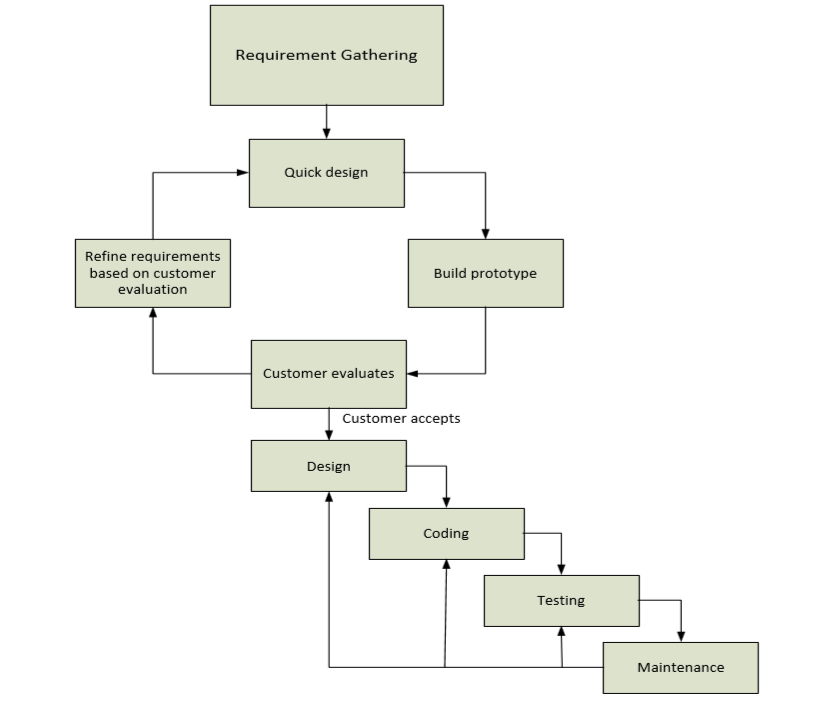
\epsfig{width=5.2in, file=Capture}
\caption{Prototype Life Cycle Model}
\end{center}
\end{figure}

\section{FEASIBILITY STUDY}
The main objective of this study is to determine whether the proposed system is feasible or not. Mainly there are three types of feasibility study to which the proposed system is subjected as described below:\\
Four key considerations are involved in this feasibility.
\begin{itemize}
\item Economic Feasibility 
\item Technical Feasibility
\item Operational Feasibility 
\item Social Feasibility
\end{itemize}
 
The proposed system must be evaluated from a technical viewpoint first, and if technically feasible, their impact on the organization must be assessed. If compatible, the operational system can be devised. Then those must be tested for economic feasibility.
\subsection{Technical Feasibility}
	The technology required for developing the driver is identified. It has technical capability to initialize the system and perform data transfer. It also provides technical guarantee of assurance, reliability, easy access and security. Thus, since both hardware and software requirements are satisfied it is technically feasible. 
\subsection{Economical Feasibility}
	The system is developed at reasonable cost with the available hardware, software and manpower. So its benefits overweigh the cost. So it is economically feasible. 
\subsection{Operational Feasibility}
The proposed project is beneficial because this driver software is the first of its class, so the users are encouraged to use it, and is expected to serve the user's needs on request. The user interface is designed in such a way that the users are not bound to have any doubts to use the interface.
\subsection{Social feasibility}
The proposed project will be socially feasible as the contents being shared is only inside a friend's circle. Such that it would not be used for any offensive purposes. The social feasibility determines whether the project would be accepted by the people. This assumption would in general examine the probability that the project would have to be accepted by the group of people that are directly affected by the proposed system.

\section{GANTT CHART}
\par Gantt chart is a graphical representation of allocation of resources to the activities. Here our resource is time. A Gantt chart is a type of bar chart that illustrates a project schedule. Gantt charts illustrate the start and finish dates of the terminal elements and summary elements of a project. Terminal elements and summary elements comprise the work breakdown structure of the project. Some Gantt charts also show the dependency (i.e., precedence network) relationships between activities. 
\par Gantt charts have become a common technique for representing the phases and activities of a project work breakdown structure (WBS), so they can be understood by a wide audience. Although a Gantt chart is useful and valuable for small projects that fit on a single sheet or screen, they can become quite unwieldy for projects with more than about 30 activities. Larger Gantt charts may not be suitable for most computer displays. A related criticism is that Gantt charts communicate relatively little information per unit area of display. That is, projects are often considerably more complex than can be communicated effectively with a Gantt chart. Although project management software can show schedule dependencies as lines between activities, displaying a large number of dependencies may result in a cluttered or unreadable chart. \\
\par Because the horizontal bars of a Gantt chart have a fixed height, they can misrepresent the time- phased work load (resource requirements) of a project, which may cause confusion especially in large projects. A related criticism is that all activities of a Gantt chart show planned workload as constant. In practice, many activities (especially summary elements) have front loaded or back-loaded work plans,so a Gantt chart with percent-complete shading actually may lead to miscommunication on the true schedule performance status.
\begin{figure}[h]
	\begin{center}
		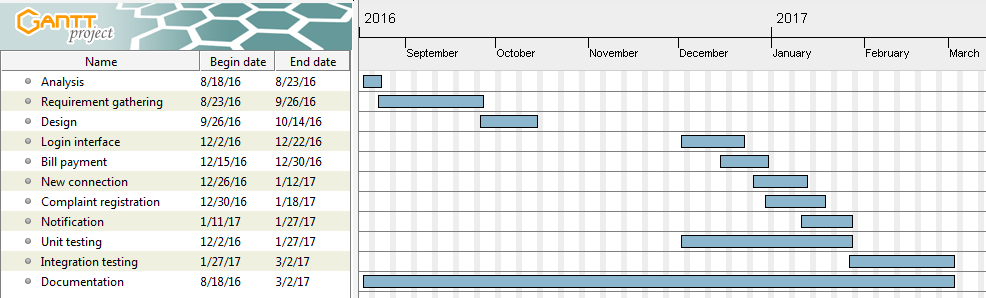
\includegraphics[width=16cm,height=7cm]{gantt.png}
			\caption{Gantt Chart}
			\label{Gantt Chart}
	\end{center}
\end{figure}
In the Gantt Chart, as per the module name each dates are given. For the feasibility study five days are given and parallel to that the requirement analysis has been started. After this comes the design phase, during this phase it took for over eighteen days for coming up with the suitable design interface according to our project. Next as a part of the implementation stage it took forty eight days for GUI development. Then comes the implementation of each modules according to our project. First in the File Insertion Module it took forty five days for its completion and for Query module it took twenty eight days and our last module that is the Text to Speech module it took twelve days for its completion. Rest comes the testing phase for double checking the performance analysis of our project by underlying them over various perspective by Unit testing, Integration testing, Final testing. At last comes the thorough documentation of each and every nook and corner of the project done, evaluated and analyzed.

\section{COST ESTIMATION}
\par Basic COCOMO computes software development effort (and cost) as a function of program size. Program size is expressed in estimated thousands of lines of code (KLOC).\\
\par COCOMO applies to three classes of software projects:\\

\begin{itemize}
\item Organic projects - \quotes{small} teams with \quotes{good} experience working with \quotes{less than rigid} requirements
\item Semi-detached - \quotes{medium} teams with mixed experience working with a mix of rigid and less than rigid requirements
\item Embedded projects - developed within a set of \quotes{tight} constraints (hardware, software, operational ...)
\end{itemize}
\par The basic COCOMO equations take the form:\\ 
\par Effort Applied = $a(KLOC)^b$[ person-months ]\\
\par Development Time = $c(Effort Applied)^d$[months]\\
\par People required = $Effort Applied / Development Time$ [count]\\
\par The coefficients a, b, c and d are given in the following table.\\
\begin{table}[!htb]
\centering
\caption{COCOMO Model Coefficients}
\label{COCOMO Model Coeffficients}
\begin{tabular}{ccccc}

\toprule
Software project & a & b & c & d\\
\midrule
\midrule
Organic   & 2.4 & 1.05 & 2.5 & 0.38\\
Semi-detached & 3.0 & 1.12 & 2.5 & 0.35\\
Embedded & 3.6 & 1.20 & 2.5 & 0.32\\
\bottomrule
\end{tabular}
\end{table}
\textit{Cost Estimation of Our Project:}\\
Effort for Development: 6PM \\
Time for development is expected to be 3 months\\
\section{SYSTEM REQUIREMENT STUDY}
\subsection{ Hardware Requirements}
 The minimum hardware specifications are:
\begin{itemize}
\item  RAM: 256MB
\item Internal memory: 40MB
\item Operating System: Android kitkat or above
\item Internet connection: 2G or above
\end{itemize}
\subsection{ Software Requirements}
\begin{itemize}
\item Tools : Android studio, Netbeans
\item Front End : Android, php, HTML 
\item Back End : MySQL
\item Platform : Android
\end{itemize}
\subsection{Safety Requirements}
\par Complete access to the system is allowed only to the administrator of this system. Clients can do nothing other than using the applications provided.\\
 
 
\chapter{SYSTEM DESIGN}
\section{DESIGN}
Design of the system includes mainly two steps:
\begin{itemize}
\item{System design}
\item{Detailed design}
\end{itemize}

 In System design a structural framework for the entire system is created. It is done in
such a way that related part come under particular groups. Thus after the system design, a
network of different groups is obtained. It is the high-level strategy for solving the problem
and building a solution. It includes the decision about the organization of the system into
subsystems, the allocation of subsystems to hardware and software components, and major
conceptual and policy decisions that form the framework for the detailed design.
\par In detailed design, each group is studied in detail and the internal operations are decided.
Based on this, the data structures and the programming language to be used are decided. Apart
from detailed design, the system design can be grouped into physical design and structural
design. The physical design maps out the details of the physical system and plans the system
implementation and specifies the hardware and software requirements.
\par Structured design is an attempt to minimize the complexity and make a problem manageable
by subdividing into smaller segments, which is called modularization or decomposition.
In this way structuring minimizes intuitive reasoning and promotes maintainable provable of systems. The structured design partitions a program into small, independent modules. They
are arranged in a hierarchy that approximates a model of the business are and is organized in a
top-down manner.
\par Logical design proceeds in a top-down manner. General features, such as reports and
inputs are identified first. Then each is studied individually and in more detail. Hence the
structured design is an attempt to minimize the complexity and make a problem.

\section{MODULES}
EBA can be divided  into the following modules.
\begin{itemize}
\item{Login interface module.}
\item{Bill payment module. }
\item{New connection module.}
\item{Complaint registration module.}
\item{Notification module.}
\subsection{Login Interface Module}
\par This feature will give the user a secure and simple login screen. The user will be provided
with a username and password by the administrator after verifying the consumer number.
\subsection{Bill Payment Module}
This feature will allow the user to pay bill online. Alerts about the last date for the bill to
be paid and previous bill payment details.
\subsection{New Connection Module}
This feature will allow the user to apply new current connection and to do other things
that are related to the current connection.
\subsection{Complaint Registration Module}
This feature will allow the user to register their complaints that are related with the current
connection.
\subsection{Notification Module}
This module will provide notifications about current connection such as power cuts, offers
from the electricity board etc.
\end{itemize}
\newpage
\section{USE CASE DIAGRAM}
\subsection{Purpose}
Use case diagram in the Unified Modeling language (UML) is a type of behavioral
diagram. Its purpose is to represent the graphical overview of the functionality provided by a
system in terms of actors, their goals (represented use cases), and any dependencies between
those use cases. The main purpose of a use case diagram is to show what system functions are
performed for which actor.\\

\subsection{Diagram}
\begin{figure}[H]
  	\begin{center}
  		\includegraphics[scale=0.38]{usecaseneweba.png}
  			\caption{Use Case Diagram}
  			\label{Use Case Diagram}
  	\end{center}
  \end{figure}
\subsection{Description}
USER:
\begin{itemize}

\item{Login to the system through the first page of the application with his/ her unique username
and password.}
\item{View notification.}
\item{Pay bill online.}
\item{Register complaints and view status.}
\item{Apply for new connection.}
\end{itemize}
SERVER:
\begin{itemize}
\item{Search the database for the details.}
\item{After successful login user can access provided features.}
\end{itemize}

\section{SEQUENCE DIAGRAM}
\subsection{Purpose}
A Sequence diagram depicts the sequence of actions that occur in a system. It portrays the
different perspectives of behavior of the system and different types of inferences can be drawn
from them. The invocation of methods in each object, and the order in which the invocation
occurs is captured in a Sequence diagram. This makes the Sequence diagram a very useful tool
to easily represent the dynamic behavior of a system.\\
\subsection{Diagram}
\begin{figure}[H]
  	\begin{center}
  		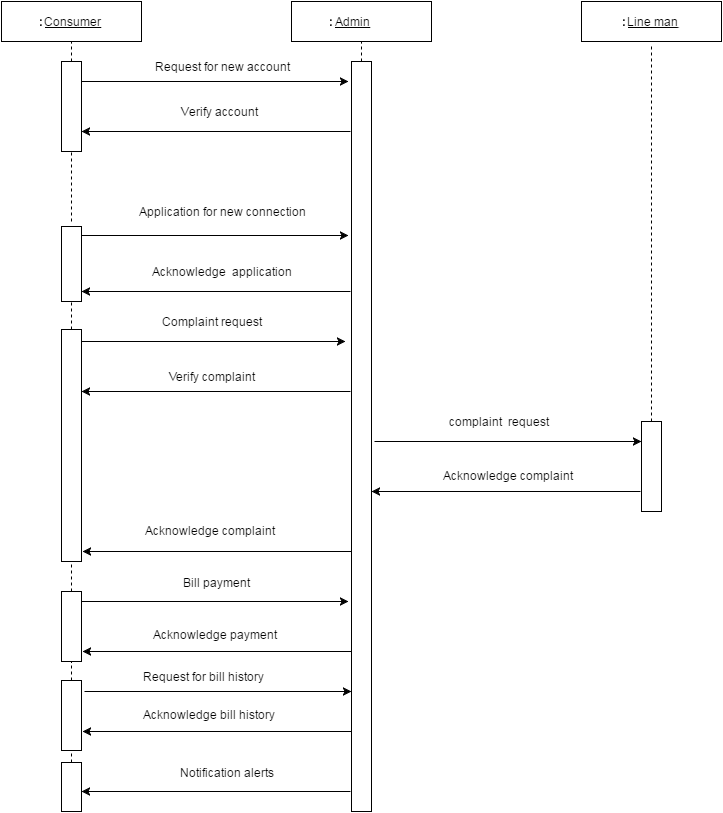
\includegraphics[scale=0.5]{sdnew.png}
  			\caption{Sequence Diagram}
  			\label{Sequence Diagram}
  	\end{center}
  \end{figure}
 \newpage
\subsection{Description}
After successful authentication with his/ her unique username and password, the user will
be able to use various features. First of all user get notification. When click pay bill option server search for the bill details from the database and show the pay options. By using complaint registration user can register complaints and can view the status related to the complaints. New connection option provide user to apply for new connection and user can view the status related to it. The action is completed when
user logout from the application.

\section{ACTIVITY DIAGRAM}
\subsection{Purpose}
The basic purpose of activity diagrams are similar to other four diagrams. It captures the dynamic behavior of the system. Other four diagrams are used to show the message flow from one object to another. But activity diagram is used to show message flow from one activity to another. Activity diagram is an important diagram in UML to describe dynamic aspects of the
system. Activity diagram is basically a flow chart to represent the flow form one activity to
another activity. The activity can be described as an operation of the system. So the control flow
is drawn from one operation to another. This flow can be sequential, branched or concurrent.
Activity diagrams deals with all type of flow control by using different elements like fork, join
etc. Activity is a particular operation of the system. Activity diagrams are not only used for visualizing dynamic nature of a system but they are also used to construct the executable system by using forward and reverse engineering technique. The only missing thing in the activity diagram is the message part,. It does not show any flow from one activity to another. Activity diagram is sometimes considered as the flow chart. Although diagram looks like the flow chart but it is not. It shows different flow like parallel, branched, concurrent and single.\\
\newpage
\subsection{Diagram}
\begin{figure}[H]
  	\begin{center}
  		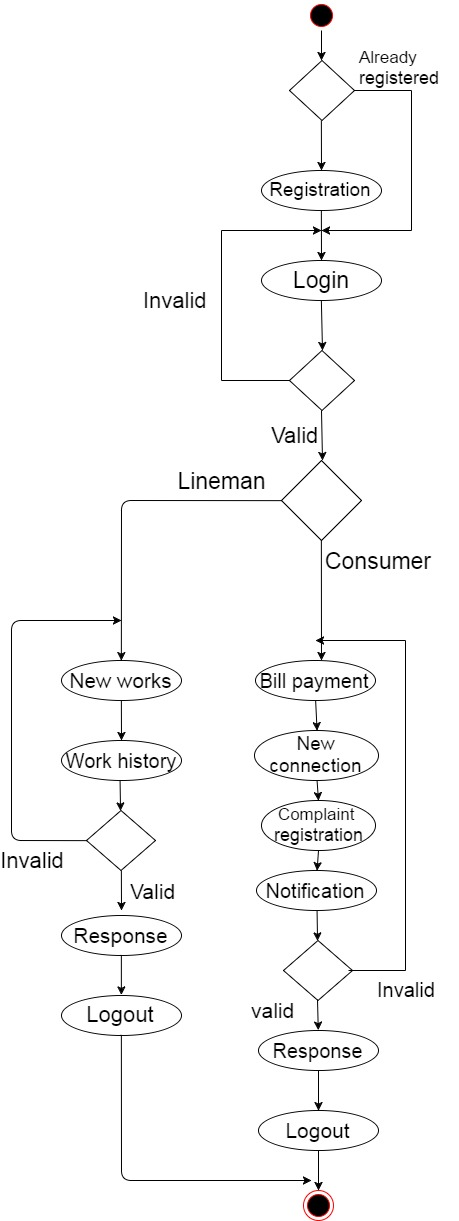
\includegraphics[scale=0.5]{actyeba.png}
  			\caption{Activity Diagram}
  			\label{Activity Diagram}
  	\end{center}
  \end{figure}
 \newpage
\subsection{Description}
\par User login to the application by using his/her user name and password. After successful login user can use various options. If the user is a new member he has to sign up using necessary informations. If the details are valid the application will give answers by searching the database. User can  logout when the actions are completed.\\ 
\newpage
\section{ER DIAGRAM}
\subsection{Purpose}
Database is recognized as a standard and is available virtually for every computer system.
The general theme behind every database is to integrate all the information. The database is an
integrated collection of data and provides centralized access to the data. The user authentication
in the project and share details is implemented using the database.
\subsection{Diagram}
\begin{figure}[h]
  	\begin{center}
  		\includegraphics[scale=0.45]{ernew1.png}
  			\caption{ER Diagram}
  			\label{ER Diagram}
  	\end{center}
  \end{figure}
  \newpage
\subsection{Description}
 The entity user has two attributes consumer number and password, where consumer number is the primary key. The application will give answer by searching the database.
\section{DATA FLOW DIAGRAM}
\subsection{Purpose}
A data flow diagram is a simple graphical formalism that represents a system in terms
of the input data to the system, various processing carried on these data, and the output data
generated by the system. A DFD model represents the data flow aspects and does not show
the sequence of execution of the different functions and conditions based on which a function
may or not be executed .In fact it completely ignores aspects such as control flow, the specific
algorithms used by the functions etc.
A DFD model uses a very limited number of primitive symbols to represent the functions
performed by the system and data flow among these functions. This network is constructed
by using a set of symbols that do not imply a physical implementation. It is a graphical tool
for structured analysis of the system requirements. DFD models a system by using external
entities, from which data flows to a process, which transforms the data and creates, output data-
flows which go to other processor or external entities or files. Data in files may also flow
to processes as inputs.\\
\\
\textbf {Notation used in data flow}
\begin{itemize}
\item\textbf{Process}
\end{itemize}
\par Process shows the work of the system. Each process has one or more data inputs and produce one or more data outputs. Processes are represented by rounded rectangles in
Data Flow Diagram. Each process has a unique name and number. This name and
number appears inside the rectangle that represents the process in a Data Flow Diagram.\\
\begin{figure}[h]
  	\begin{center}
  	
  	
  		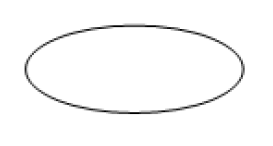
\includegraphics[width=3 in,height=1 in]{ellipse.png}
  			\end{center}
  \end{figure}
  \\
  \begin{itemize}
  \item\textbf{Data Stores}
  \end{itemize}
\par A data store is a repository of data. Processes can enter data, into a store or retrieve the
data from the data store. Each data has a unique name.\\
\begin{figure}[h]
  	\begin{center}
  	
  	
  		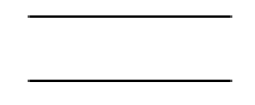
\includegraphics[width=3 in,height=1 in]{process.png}
  			\end{center}
  \end{figure}
  
  \begin{itemize}
  \item\textbf{Data Flows}
  \end{itemize}
  \par Data flows show the passage of data in the system and are represented by lines joining
  system components. An arrow indicates the direction of flow and the line is labeled by
  name of the data flow.\\
  
  \begin{figure}[h]
    	\begin{center}
    	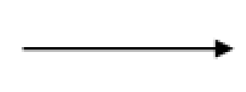
\includegraphics[width=3 in,height=1 in]{data.png}
    			\end{center}
    \end{figure}
 \newpage
 \begin{itemize}
 \item\textbf{External Entity}
 \end{itemize}
 \par External entities are outside the system but they either supply input data into the system or
 use other systems output. They are entities on which the designer has control. They may
 be an organizations customer or other bodies with which the system interacts. External
 entities that supply data into the system are sometimes called source. External entities that use the system data are sometimes called sinks. These are represented by rectangles
 in the Data flow Diagram.\\
 
 \begin{figure}[h]
   	\begin{center}
   	
   	
   		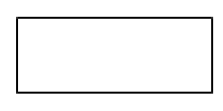
\includegraphics[width=3 in,height=1 in]{ex.png}
   			\end{center}
   \end{figure}

\textbf{LEVEL 0}

\begin{figure}[h]
  	\begin{center}
  		\includegraphics[scale=0.5]{level0.png}
  			\caption{Level 0 DFD}
  			\label{Level 0 DFD}
  	\end{center}
  \end{figure}
  \textbf{Description}
  \\
  \par User can request to Electricity Board Application, it will respond to the user.\\
  \newpage
  \textbf{LEVEL 1}
  
  \begin{figure}[h]
    	\begin{center}
    		\includegraphics[scale=0.48]{level1.png}
    			\caption{Level 1 DFD}
    			\label{Level 1 DFD}
    	\end{center}
    \end{figure}
    
    \textbf{Description}
    \\
    \par User can login to the website using user name and password. After successful login user
    can request for bill payment, new connection, complaint registration and notification. Then
    EBA will respond to the request asked by the user.\\
  \newpage  
    \textbf{LEVEL 2}
      
      \begin{figure}[h]
        	\begin{center}
        		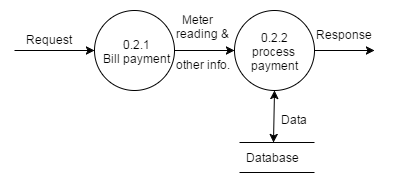
\includegraphics[scale=1.2]{level21.png}
        			\caption{Level 2.1 DFD}
        			\label{Level 2 DFD}
        	\end{center}
        \end{figure}
      \begin{figure}[h]
              	\begin{center}
              		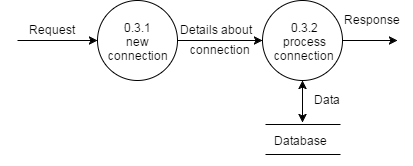
\includegraphics[scale=1.2]{level22.png}
              			\caption{Level 2.2 DFD}
              			\label{Level 2 DFD}
              	\end{center}
              \end{figure}  
       \begin{figure}[h]
               	\begin{center}
               		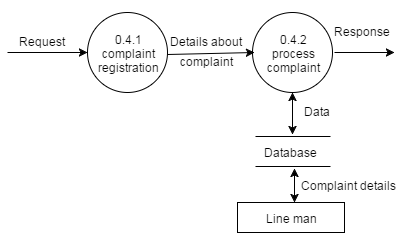
\includegraphics[scale=1.2]{level23.png}
               			\caption{Level 2.3 DFD}
               			\label{Level 2.3 DFD}
               	\end{center}
               \end{figure}
       \begin{figure}[h]
               	\begin{center}
               		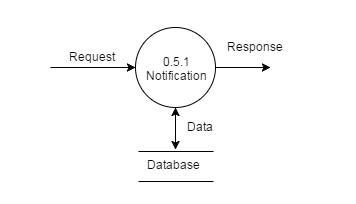
\includegraphics[scale=1.2]{level24.png}
               			\caption{Level 2.4 DFD}
               			\label{Level 2 DFD}
               	\end{center}
               \end{figure}         
        \textbf{Description}
        \par When the user request an option, then EBA will process the request with the help of
        database if necessary, where the data are stored. By using the appropriate data from the database.
 \chapter{IMPLEMENTATION}
 \par Implementation is the stage in the project where the theoretical design is turned into a working system and is giving confidence on the new system for users that it will work effectively and effectively. It involves careful planning, investigation of the current system and it constraints on implementation, design of achieve the changeover, an evolution of change over method. A part from planning major task of preparing the implementation are education and training of users .The more complex system being implemented, the more involved will be the system analysis and the design effort required just for implementation.\\
 \par  The product is developed in Python environment in windows platform. This chapter may explain our implementation details.\\
 \section{ LANGUAGES AND PLATFORM USED}
\par Implementation is the stage in the project where the theoretical design is turned into a
working system and is giving confidence on the new system for users that it will work effectively.
It involves careful planning, investigation of the current system and it constraints
on implementation, design of achieve the changeover, an evolution of change over method.
The application is developed in android environment. The tools used for the development are
JAVA,PHP,ANDROID and MySQL for the database.\\

\subsection{Android}
Android is an operating system based on the kernel, and designed primarily for touch screen mobile devices such as smart phones and tablet computers. Initially developed by Android, Inc., which Google backed financially and later bought in 2005,Android was unveiled in 2007 along with the founding of the Open Handset Alliance a consortium of hardware, software, and telecommunication companies devoted to advancing open standards for mobile devices. The first publicly available smartphone running Android, the HTC Dream, was released on October 22, 2008.
 
 
\par
Android offers a number of features to developers:
\begin{itemize}
\item Storage : Uses SQLite, a lightweight relational database, for data storage
\item Connectivity: Supports  GSM/EDGE,  IDEN,  CDMA,  EV-DO,  UMTS,  Bluetooth  (includes  A2DP  and

AVRCP), Wi-Fi, LTE, and WiMAX.
\item Messaging: Supports both SMS and MMS
\item Web browser: Based on the open-source Web Kit, together with Chrome’s V8 JavaScript engine.
\item Media Support: Includes support for the following media: H.263, H.264 (in 3GP or MP4 container), MPEG-4

SP, AMR, AMR-WB (in 3GP container), AAC, HE-AAC (in MP4 or 3GP container), MP3, MIDI, Ogg

Vorbis, WAV, JPEG, PNG, GIF, and BMP.
\item Hardware support: Accelerometer Sensor, Camera, Digital Compass, Proximity Sensor, and GPS
\item Multi-tasking:Supports multi-tasking applications
\item  Tethering : Supports sharing of Internet connections as a wired/wireless hotspot

\end{itemize}


\subsubsection{Architecture}
\begin{figure}[h]
\begin{center}
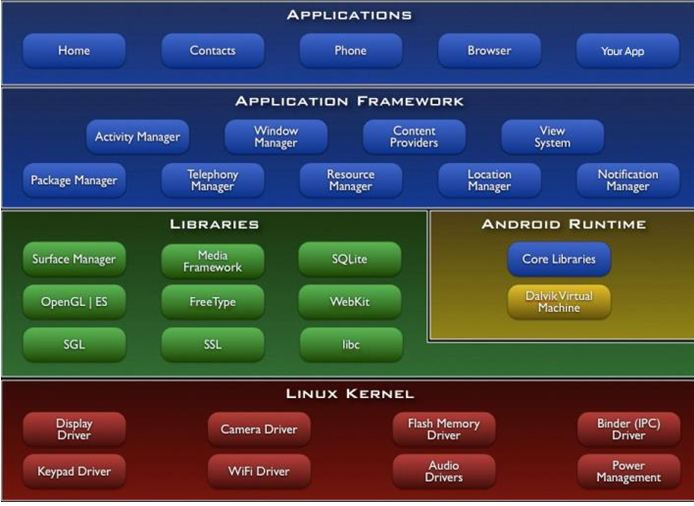
\includegraphics[width=.7\textwidth]{arch.jpg}
\caption{Architecture of Android}
\end{center}
\end{figure}

The above figure shows the diagram of Android Architecture. The Android OS can be referred to as a software stack of different layers, where each layer is a group of several program components. Together it includes operating system, middleware and important applications. Each layer in the architecture provides different services to the layer just above it

\par
The basic layer is the Linux kernel. The whole Android OS is built on top of the Linux 2.6 Kernel with some further architectural changes made by Google. It is this Linux that interacts with the hardware and contains all the essential hardware drivers. Drivers are programs that control and communicate with the hardware. For example, consider the Bluetooth function. All devices has a Bluetooth hardware in it. Therefore the kernel must include a Bluetooth driver to communicate with the Bluetooth hardware. The Linux kernel also acts as an abstraction layer between the hardware and other software layers. Android uses the Linux for all its core functionality such as Memory management, networking, security settings etc. As the android is built on a most popular and proven foundation, it made the porting of Android to variety of hardware, a relatively painless task.

\subsubsection{Versions Of Android}
\begin{itemize} 
\item Android 1.0
\item	Android 1.1
\item	Android 1.5 - Cupcake
\item	Android 1.6 - Donut
\item	Android 2.0/2.1 - Éclair
\item	Android 2.2 - Froyo
\item	Android 2.3 - Gingerbread
\item	Android 3.0 - Honeycomb
\item	Android 4.0 - Ice-cream Sandwich
\item	Android 4.1 - Jellybean
\item	Android 4.4 - Kit Kat
\item	Android 5.0 – Lollipop
\item	Android 6.0 - Marshmallow
\item	Android 7.0 - Noughat

\end{itemize}


\subsection{Java}
Java is a general-purpose computer programming language that is concurrent, class based,
object-oriented, and specifically designed to have as few implementation dependencies
as possible. Java applications are typically compiled to byte code that can run on any Java
virtual machine (JVM) regardless of computer architecture. The syntax of Java is largely influenced
by C++. Unlike C++, which combines the syntax for structured, generic and object-oriented
programming. Java was built almost exclusively as an object-oriented language. All
code is written inside classes, and every data item is an object, with the exception of the primitive
data types, i.e. integers, floating-point numbers, boolean values and characters, which are
not objects for performance reasons.
\subsection{PHP}
PHP is a server-side scripting language designed primarily for web development but
is also used as a general-purpose programming language. PHP code may be embedded into
HTML code, or it can be used in combination with various web template systems, web content
management systems and web frameworks. Many fatal- or recoverable-level legacy PHP error
mechanisms were replaced with modern object-oriented exceptions. In terms of keywords and
language syntax, PHP is similar to the C style syntax. If conditions, for and while loops, and
function returns are similar in syntax to languages such as C, C++,Java and Perl.


 \section{METHOD OF IMPLEMENTATION}
 \par EBA is an android application with its server developed in PHP and database in MySQL. The android application is used by the consumers and the linemen. For the administrative view there is a web side view which is done in HTML and CSS used for styling. XAMPP provides support for creating and manipulating database in MySQL. Once XAMPP is installed it is possible to treat a localhost like a remote host by connecting to it. The PHP coding was done in Netbeans IDE. This platform offers reusable services, allowing developers to focus on the logic specific to their applications. 
 \par In the android application after the splash screen shows up two gateways to consumer and lineman. Once the consumer is selected, the next page is to insert the username and password and then login to the respected consumer accounts. There is also a facility to sign up for a new account which requires name, address, phone no, consumer no, username and password for the sign up process. Once a consumer is logged in to their account, the main page shows the notifications which includes notifications regarding bills, current cuts, current connection etc.. Then on the navigation drawer there are selections for bill payment, bill history, apply new connection, application status, complaint, complaint status, change password, help and calendar.
 In the bill payment user can review the present bill and can pay the bill online either using credit or debit cards. On the bill history page all the information regarding the bills for that respected consumer can be seen and viewed in detail. For applying a new connection one can fill up the application form online and can check status through the application itself. Complaint can be booked through the application, details of the consumers post no, transformer no or section no need not be provided, unless if some other spot have to be complainted. Complaint status for each of the complaints booked by the respective user can also be viewed. Change Password screen provides a user to change his password. One should insert the old password and the new password twice for changing the password. Help screen shows a basic idea for using the application.
 \par When lineman is selected, one can login to the account only by using a verified lineman's employee number and their respected password. Once logged in the first page shows the all those works to be done by the respected lineman. For simplicity color representation are given such that, red color marks the new works not yet viewed by the lineman, yellow color shows the works attending and the blue color shows works that are under progress. On clicking the work, a new page opens up showing the details of the complaint and contains three buttons for updating the status as attending, completed and progress. To go back the lineman can click anywhere in the page. There is also facility to know the details of those works which are already completed by the respected lineman logged in. Those works shown in color yellow hints that the work was completed but not by the lineman logged in. The process of changing password remains the same as that in consumer.
 \par The Administrative process are to be done by accessing the index page. The credentials if provided correctly will show up the home page. In home page there is a simple clock and the logo. From the above dropdown menu administrator can select the modules. The Drop down lists include Lineman add, which is used to add a lineman to the database which contains the employee number, name, section number and password for which the field left empty the default password would be 'password'. Lineman details show all linemen that are added in the database, on clicking the name of the lineman, whole works that are sent to his/her databse is shown with color representations such that green, indigo, blue, yellow, red as completed, completed by co worker, progress, attending and unseen as the status respectively. Admin also have the privilage to change the name of a lineman or to terminate a lineman. There is apage which shows all those new application requests for current connection and facility to update status or to approve the application, if approved the admin should provide details of each user with consumer no, section no, post no, tranformer no etc. Verified consumers can be accessed through another page and the admin can check the full details of the consumer by clicking their respected names. There is also a bill history details of the consumer selected in the same page. The details of each and every users signed up for the EBA application can be viewed throught the EBA users page. The Notifications page provide an input field for the admin to broadcast a notification such that if the section no is provided as 0, the notification is provided to all the users and if provided with an explicit section no, then those consumers who belongs to that repsected section no will recieve that notification. Administrator can also view all the notifications broadcasted yet to date and have privilage to delete any notifications from the database. Complaint page provide information about each and every complaints recived up to date. The admin can also view those linemen that are working for the complaint. Admin can even add new lineman for a complaint work. Admin can also view all those details of the complaints that are already fixed in History page. Update Bill page provides the admin to insert the current meter reading of the month for each consumer, and the program will automatically calculate the bill amount and notifications to each and every consumer will be broadcasted and the new bill will be shown. Bill due page shows the details of those consumers who have not yet paid the bill for the current month. Once the admin logout from the page, the sessions variable will reset, hence one cannot access the page with only the link.
 
\newpage
\section{SCREENSHOTS}
\subsection{Welcome page}
\begin{figure}[H]
	\begin{center}
		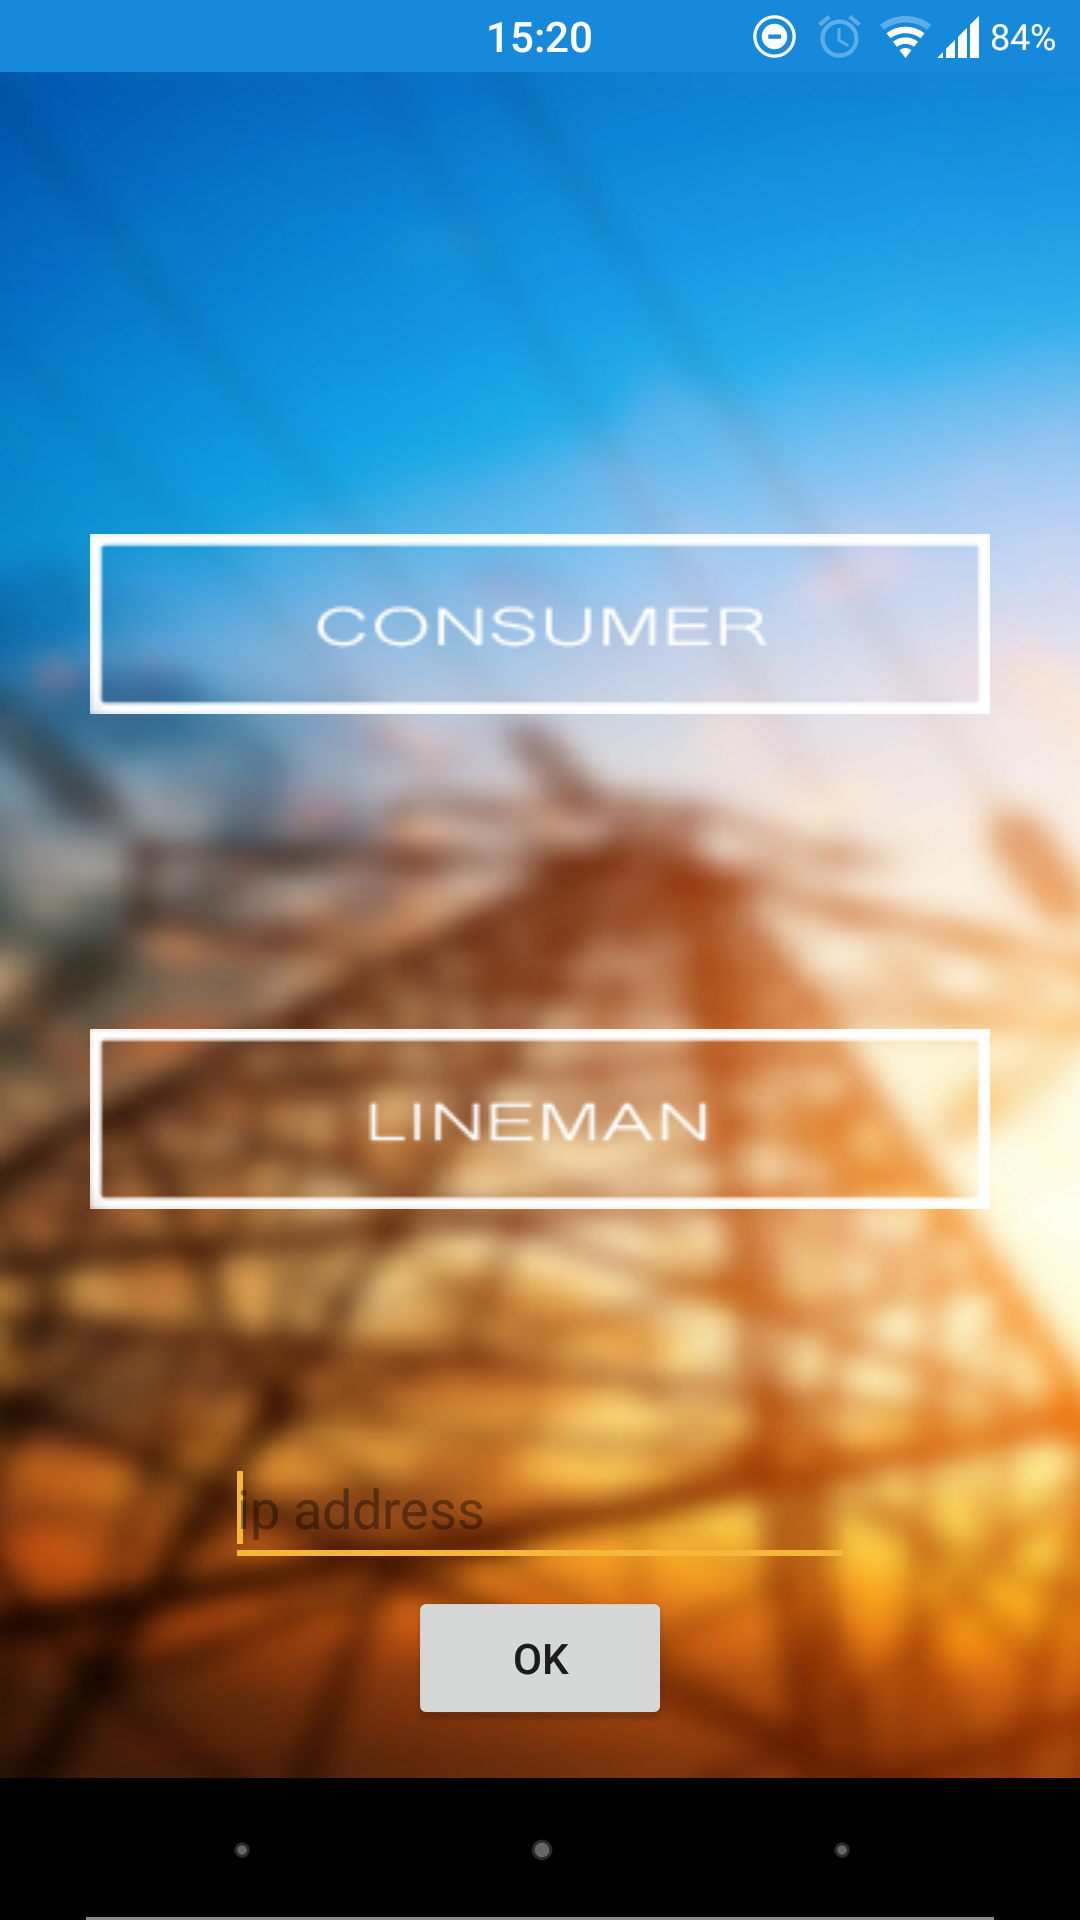
\includegraphics[width=7cm,height=12cm]{startup.png}
			\caption{Welcome page}
			\label{Welcome page}
	\end{center}
\end{figure}
\textbf{Description}
\par A link to the consumer and lineman page is also provided in this page. So EBA user can easily select two accounts.

\newpage
\subsection{Sign Up}
\begin{figure}[H]
	\begin{center}
		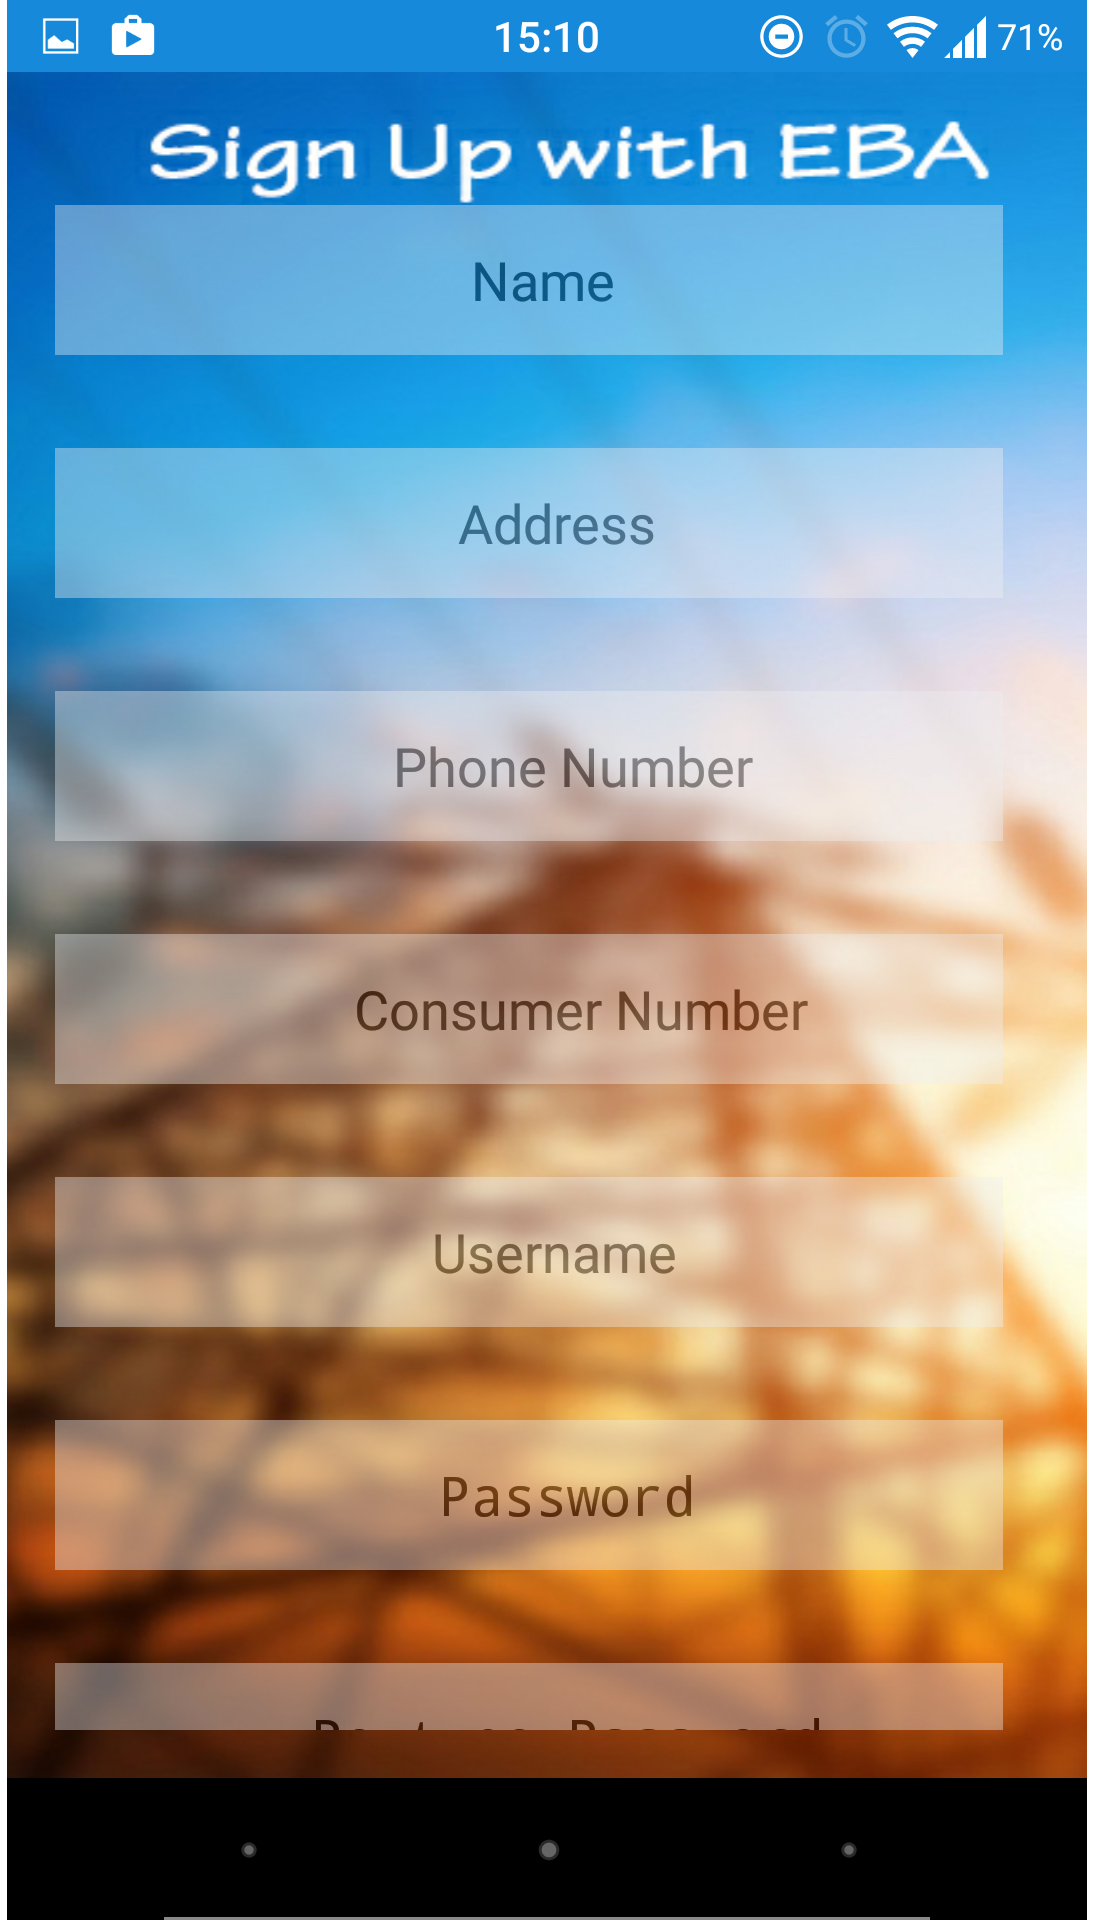
\includegraphics[width=7cm,height=12cm]{signupss.jpg}
			\caption{Sign Up page}
			\label{Sign Up page}
	\end{center}
\end{figure}
\textbf{Description}
\par This page is used for a new registration. The page includes the basic informations for the registration of a new user such as name, password, consumer number.
\newpage
\subsection{Sign In}
\begin{figure}[h]
	\begin{center}
		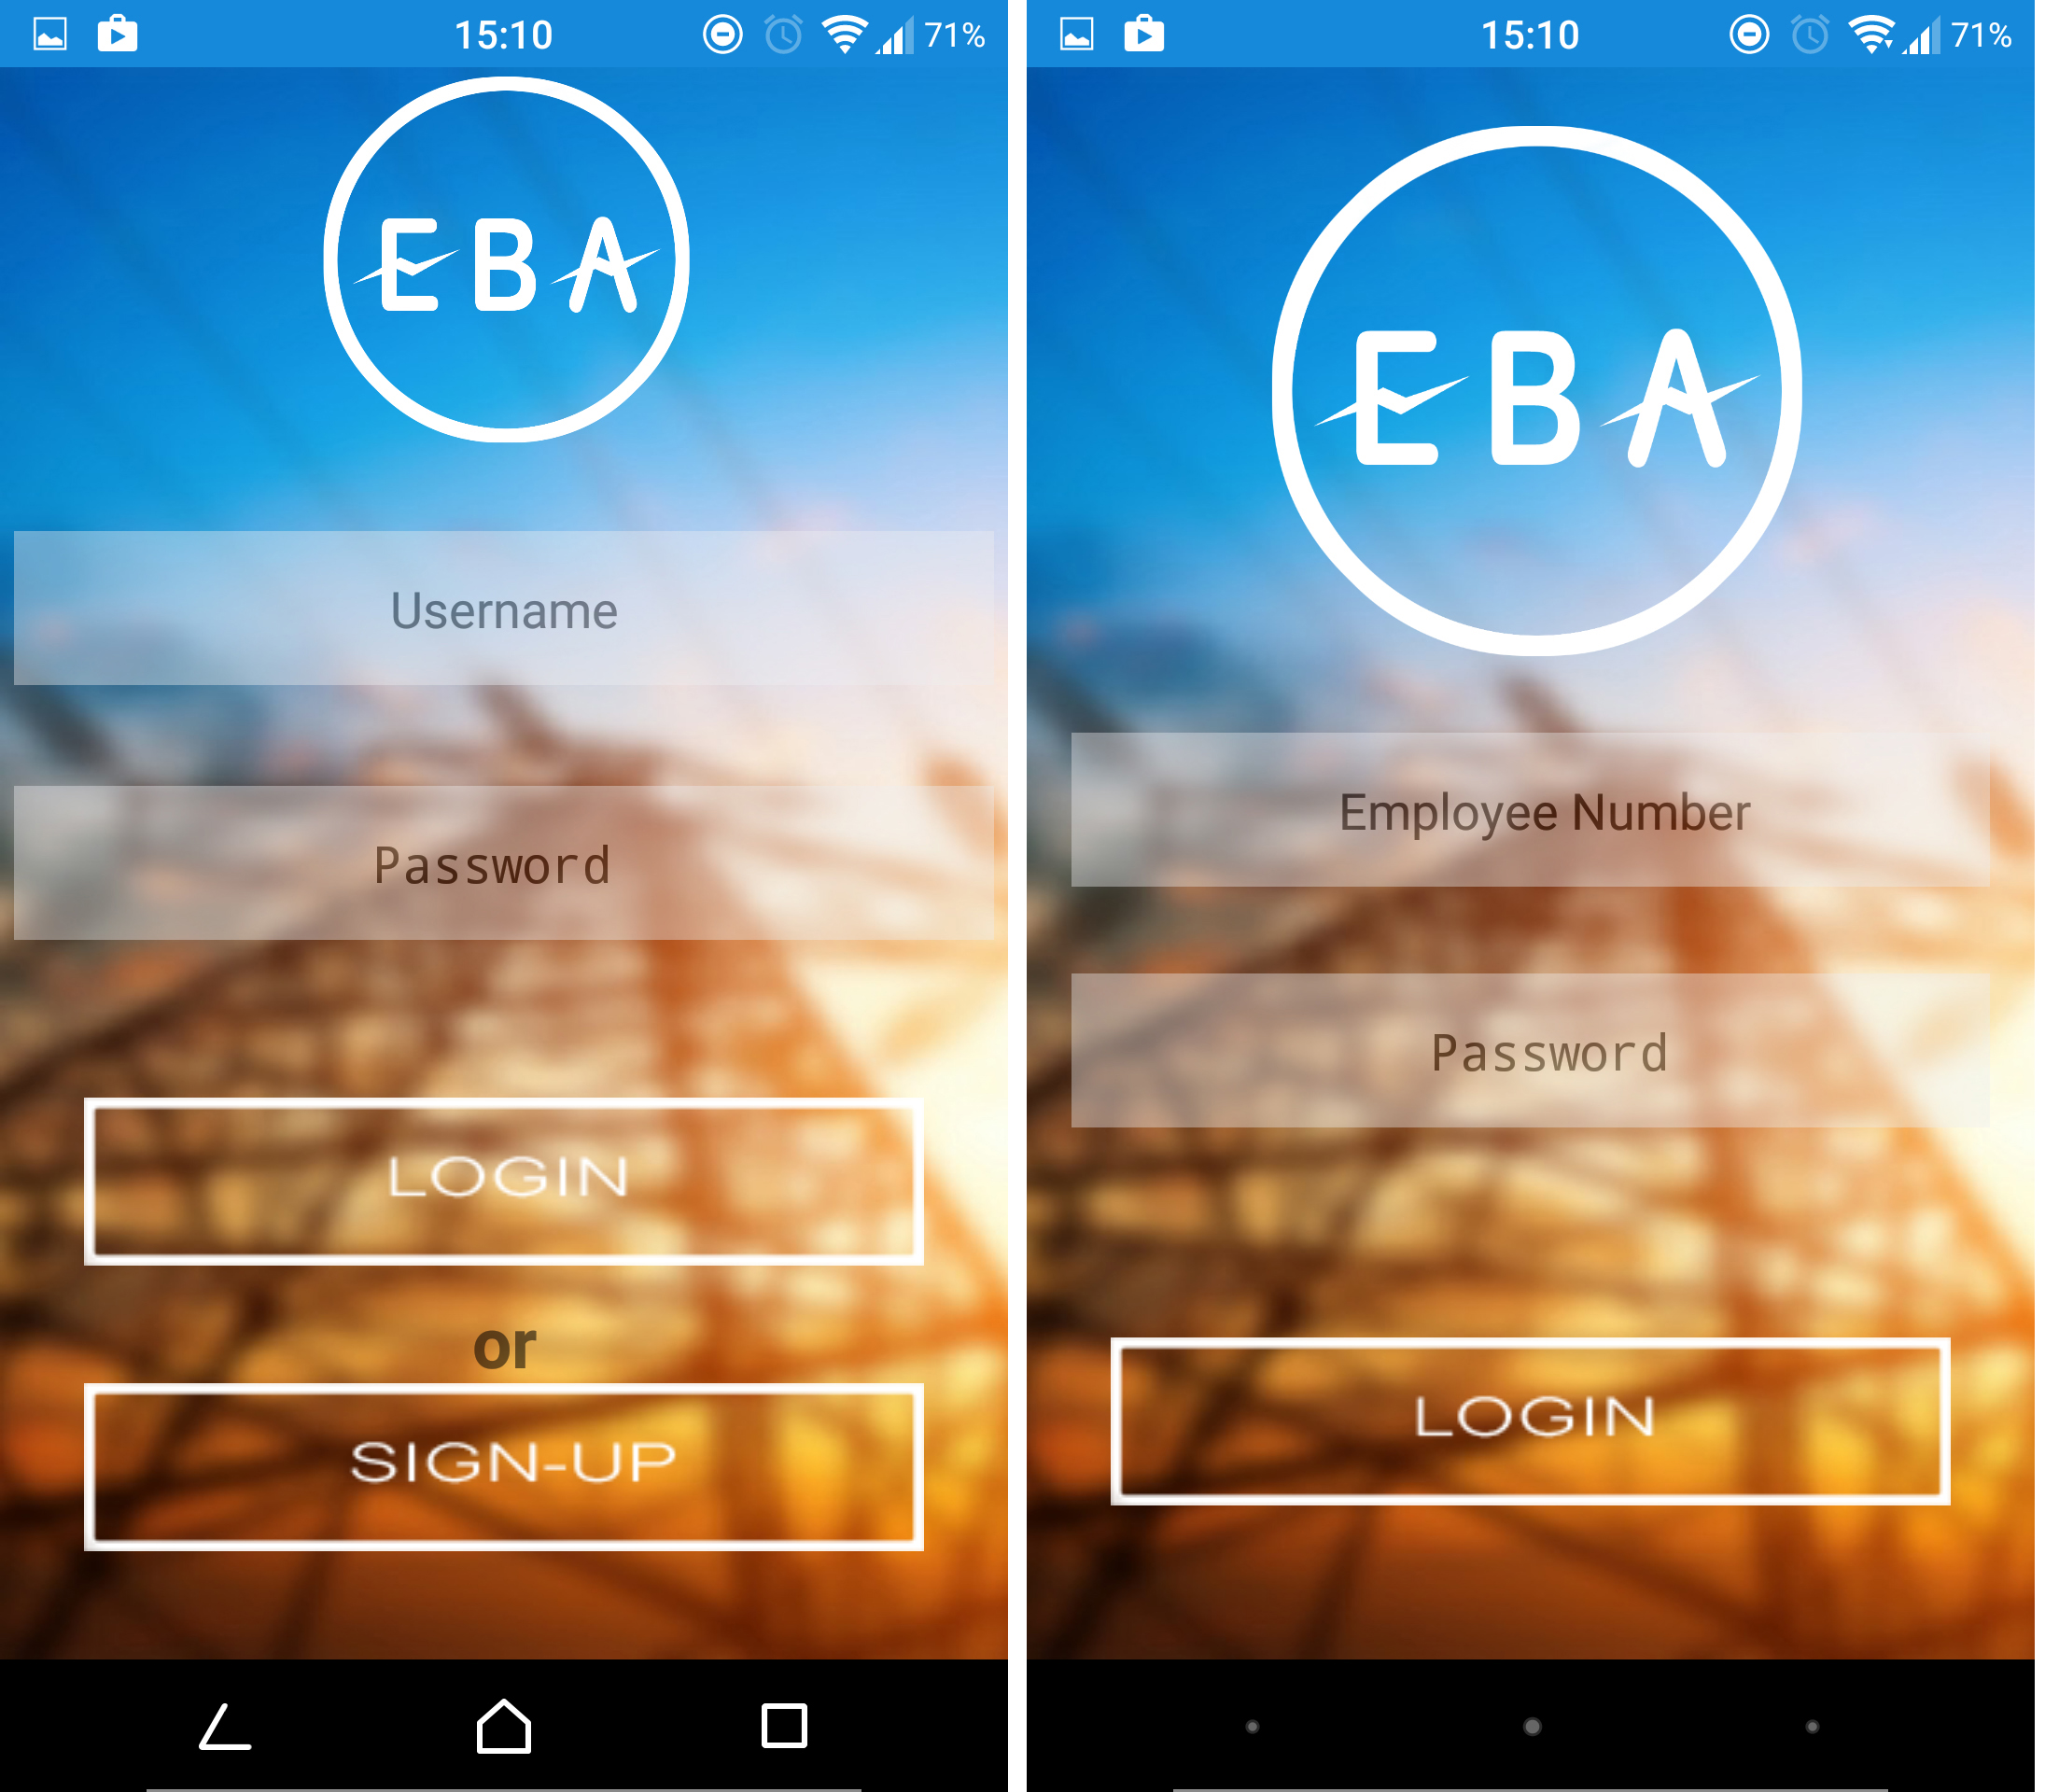
\includegraphics[width=12cm,height=10cm]{sslogin.jpg}
			\caption{Sign In page}
			\label{Sign In page}
	\end{center}
\end{figure}
\textbf{Description}
\par The sign in page consists of two text fields where the users need to enter their login credentials to login to EBA.

\newpage
\subsection{Home screen of consumer}
\begin{figure}[h]
	\begin{center}
		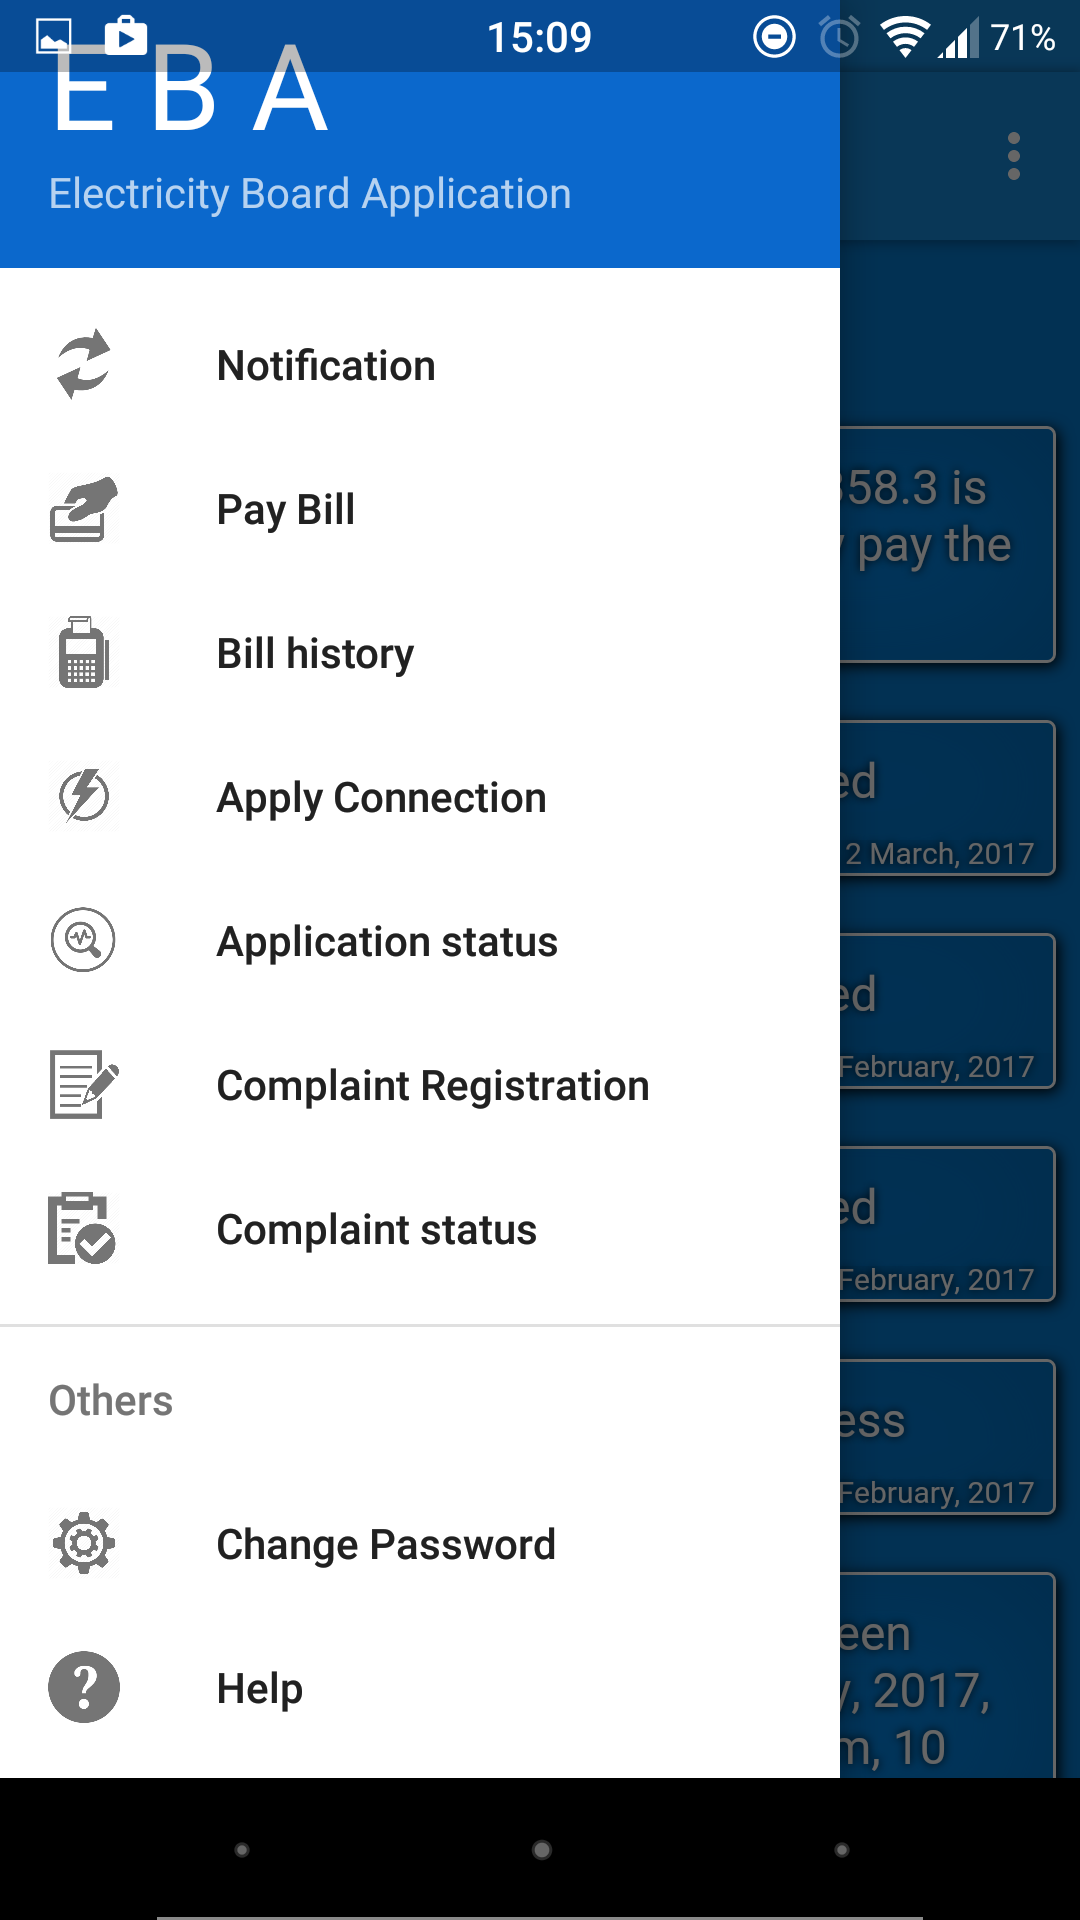
\includegraphics[width=7cm,height=12cm]{homepage.png}
			\caption{Home page}
			\label{Home page}
	\end{center}
\end{figure}
\textbf{Description}
\par This page has several choices. Those are notification, pay bill, bill history, apply connection, application status, complaint registration, complaint status, change password and help.


\newpage
\subsection{Notification and Bill payment}
\begin{figure}[h]
	\begin{center}
		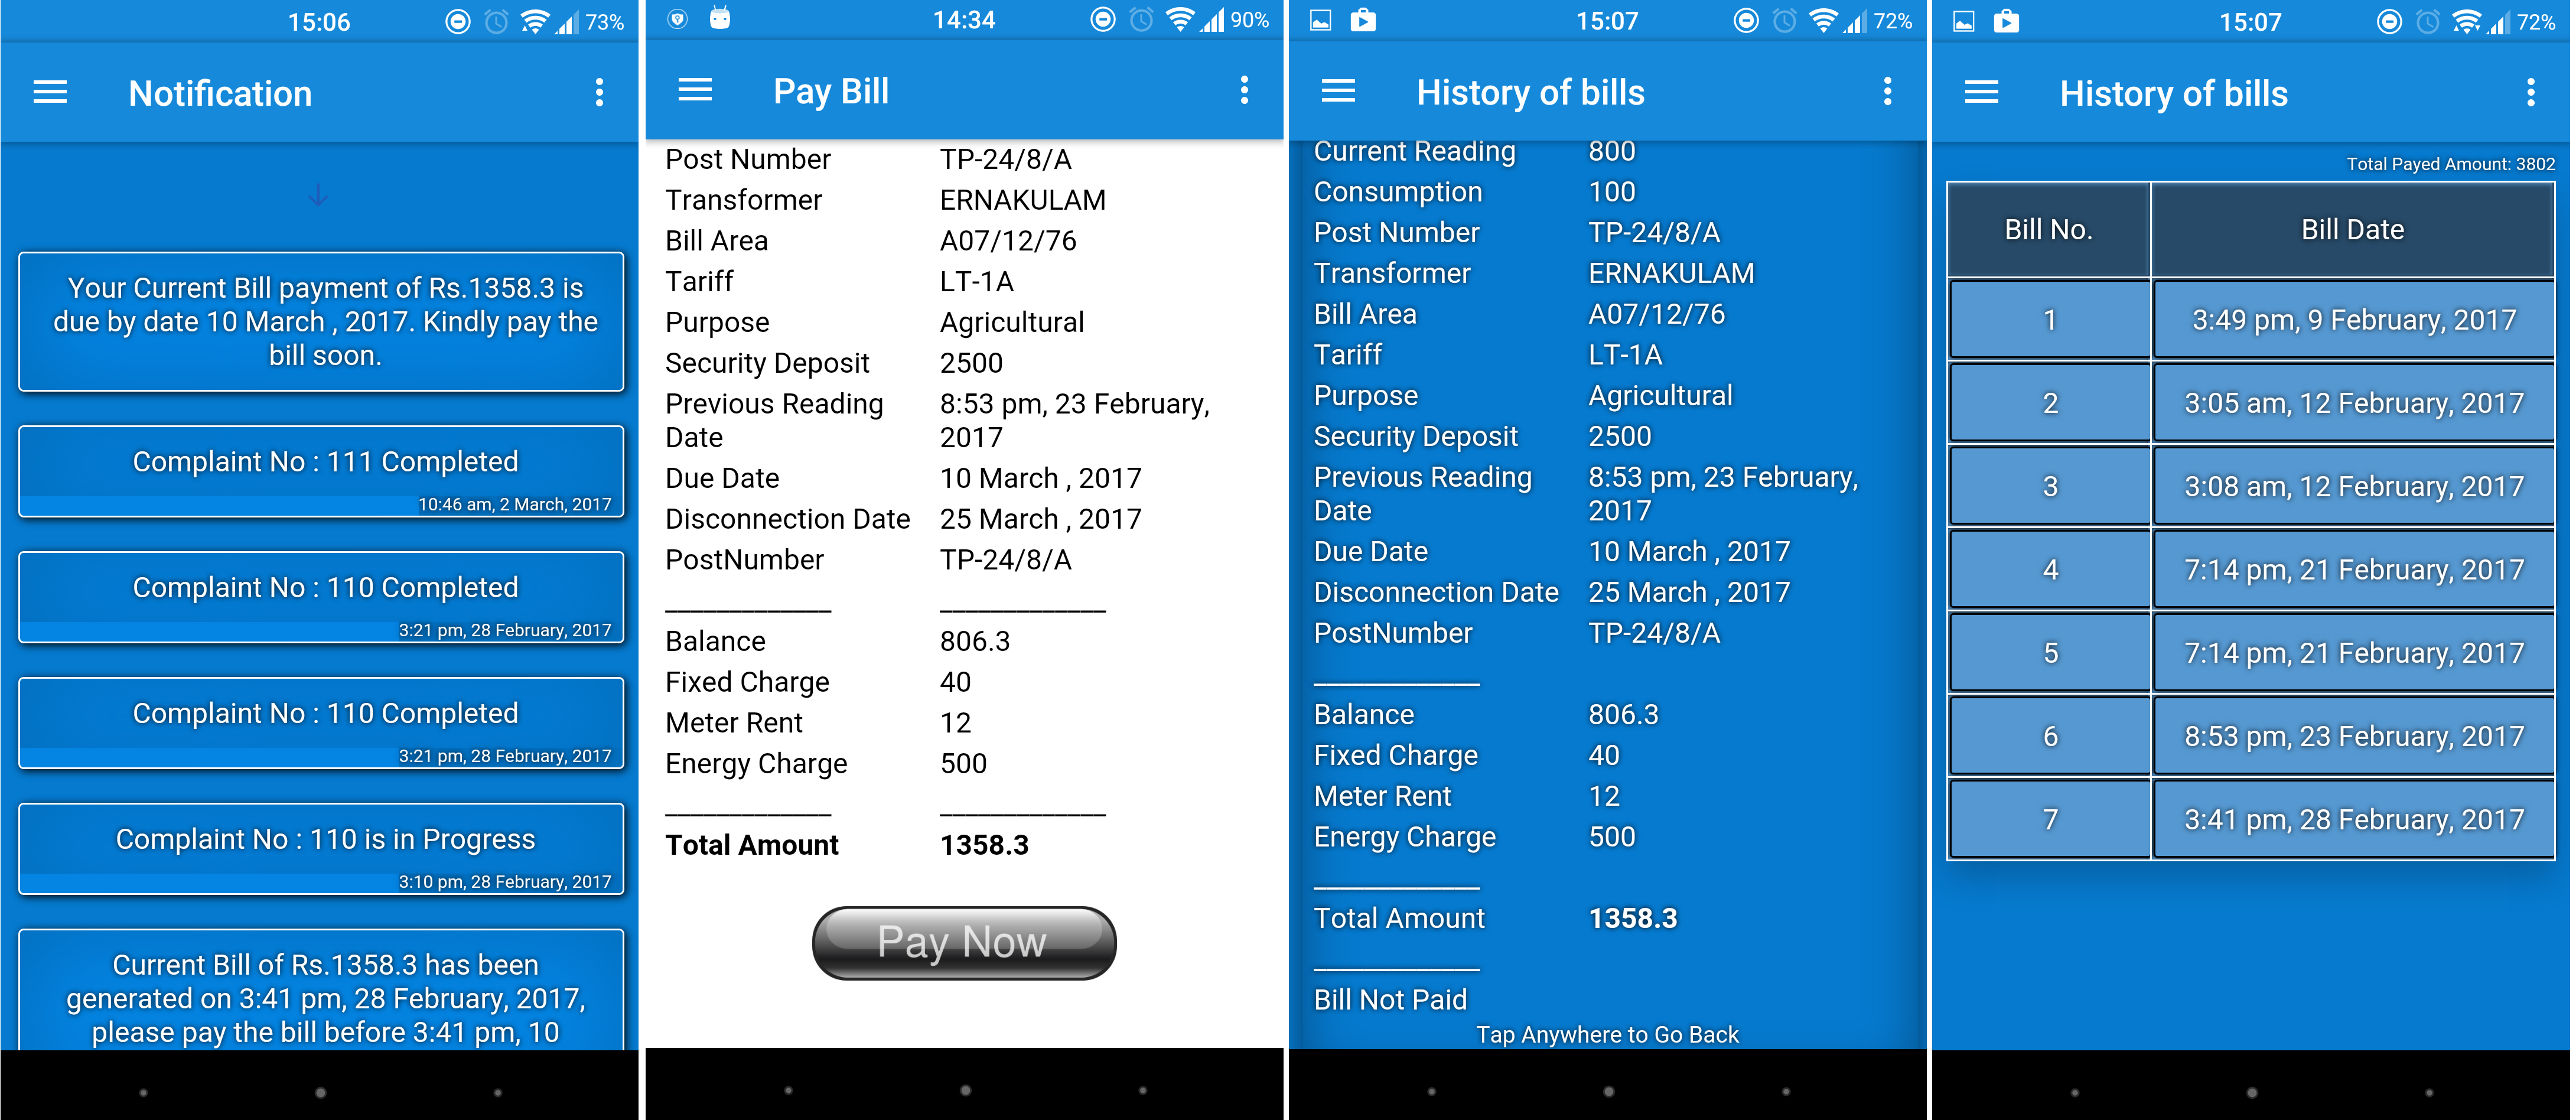
\includegraphics[scale=0.07]{billhis.jpg}
			\caption{Notification and Bill payment}
			\label{Notification and Bill payment}
	\end{center}
\end{figure}
\textbf{Description}
\par From the notification page we can view notification from the Electricity board. And from the bill payment page we can pay electricity bill online and view the previous bill details.

\newpage
\subsection{New connection and Complaint registration}
\begin{figure}[H]
	\begin{center}
		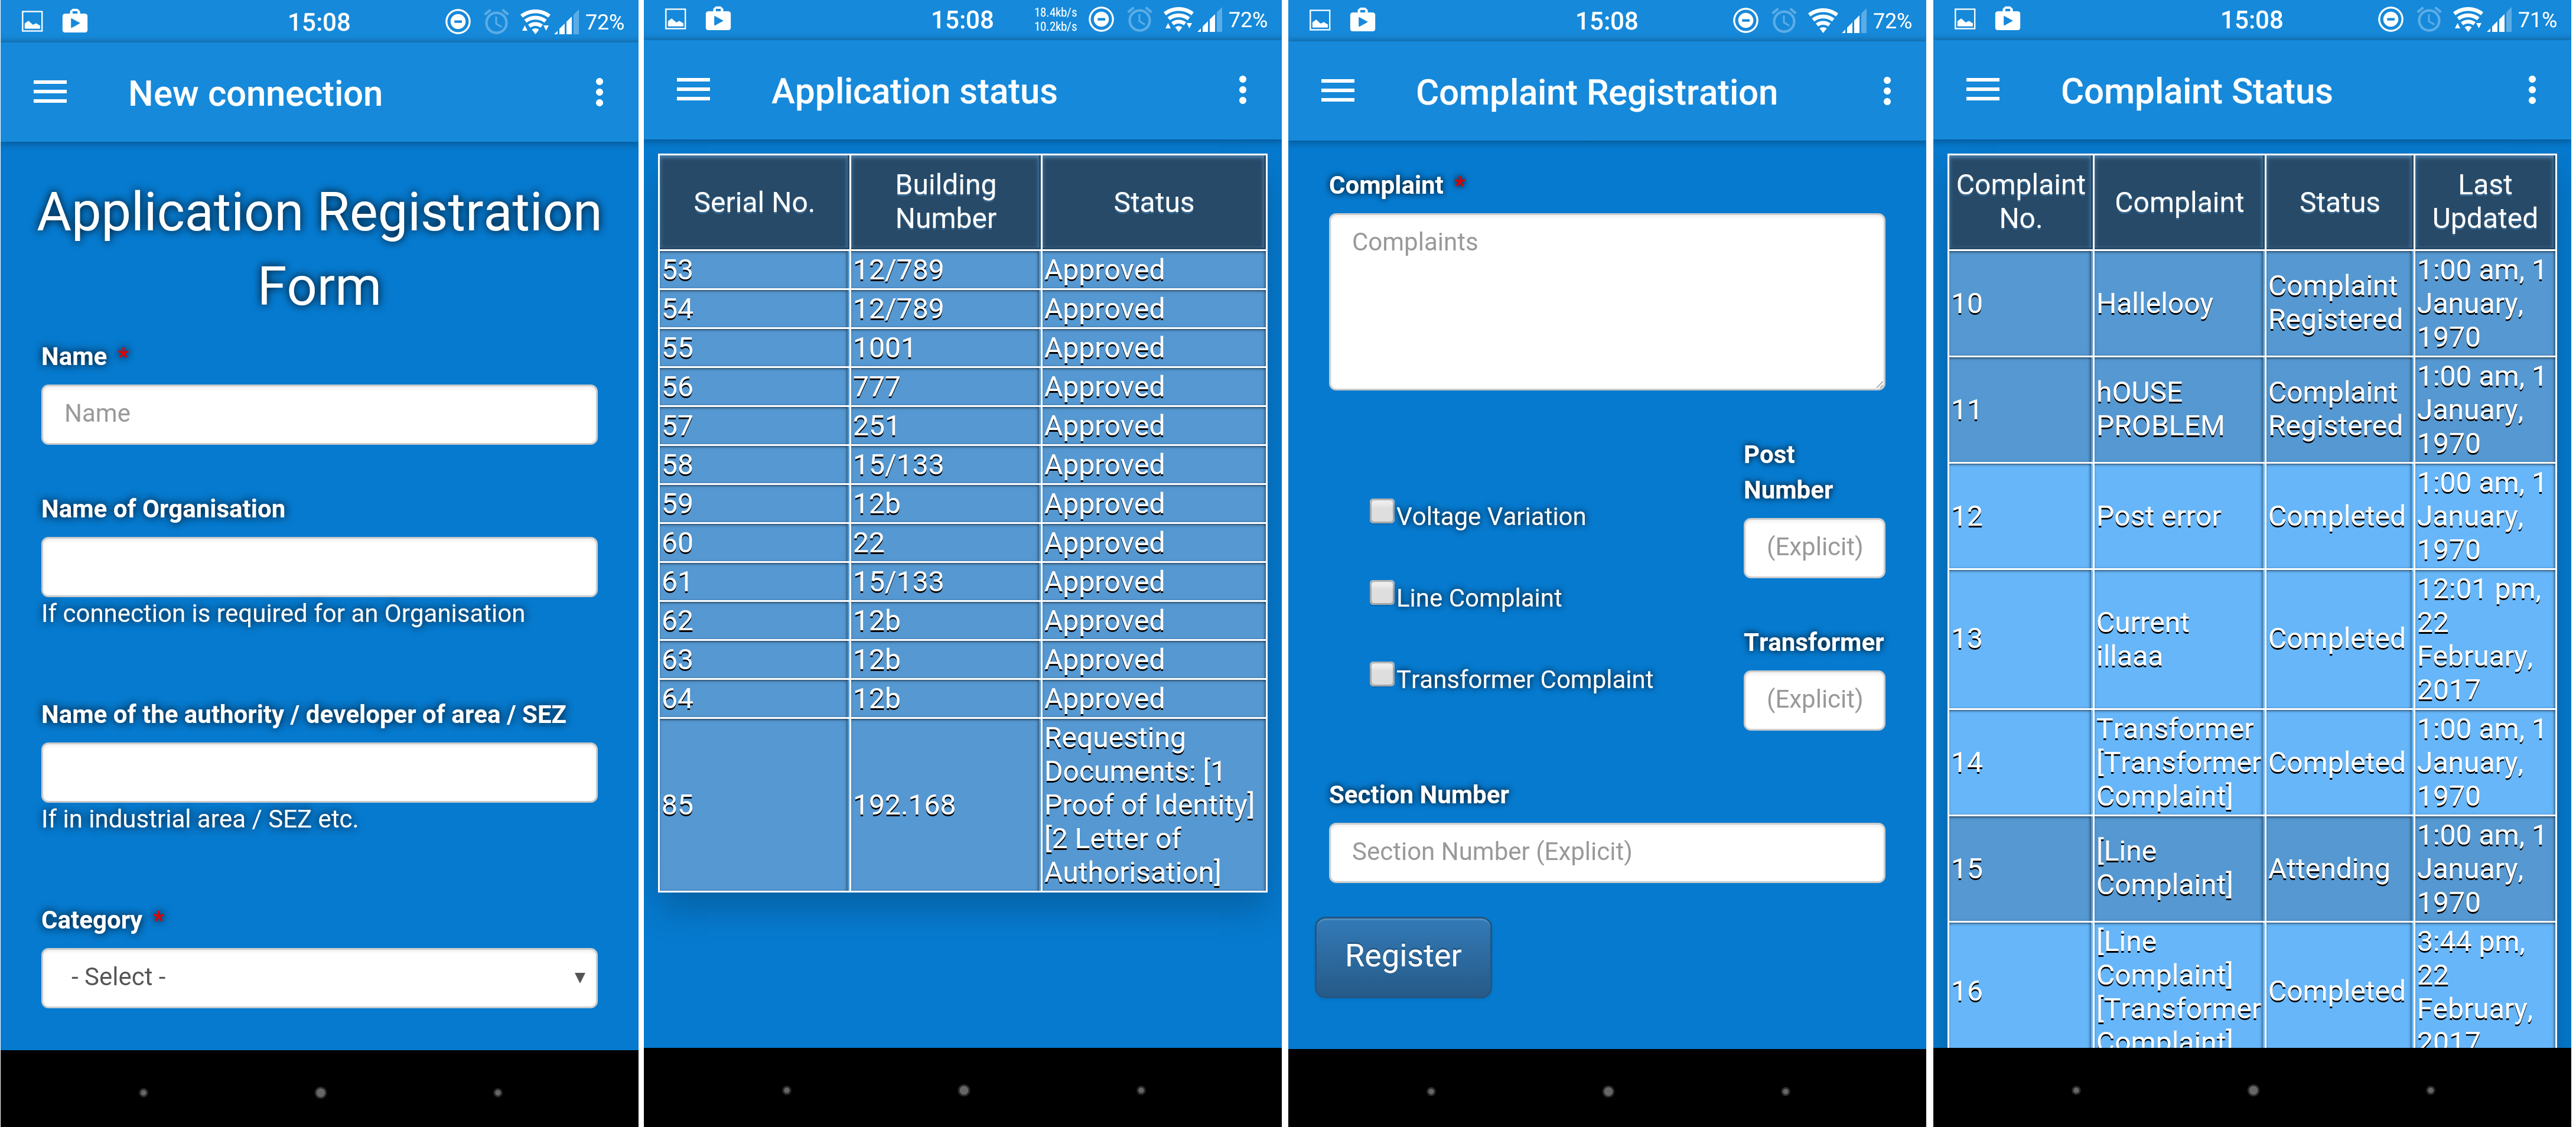
\includegraphics[scale=0.07]{newcompl.jpg}
			\caption{New connection and complaint registration}
			\label{New connection and complaint registration}
	\end{center}
\end{figure}
\textbf{Description}
\par Through new connection page user can apply for new connection and view those status.
 In complaint registration page user can register their complaints about the current connection and view complaint status.

\newpage
\subsection{Change password and Help}
\begin{figure}[h]
	\begin{center}
		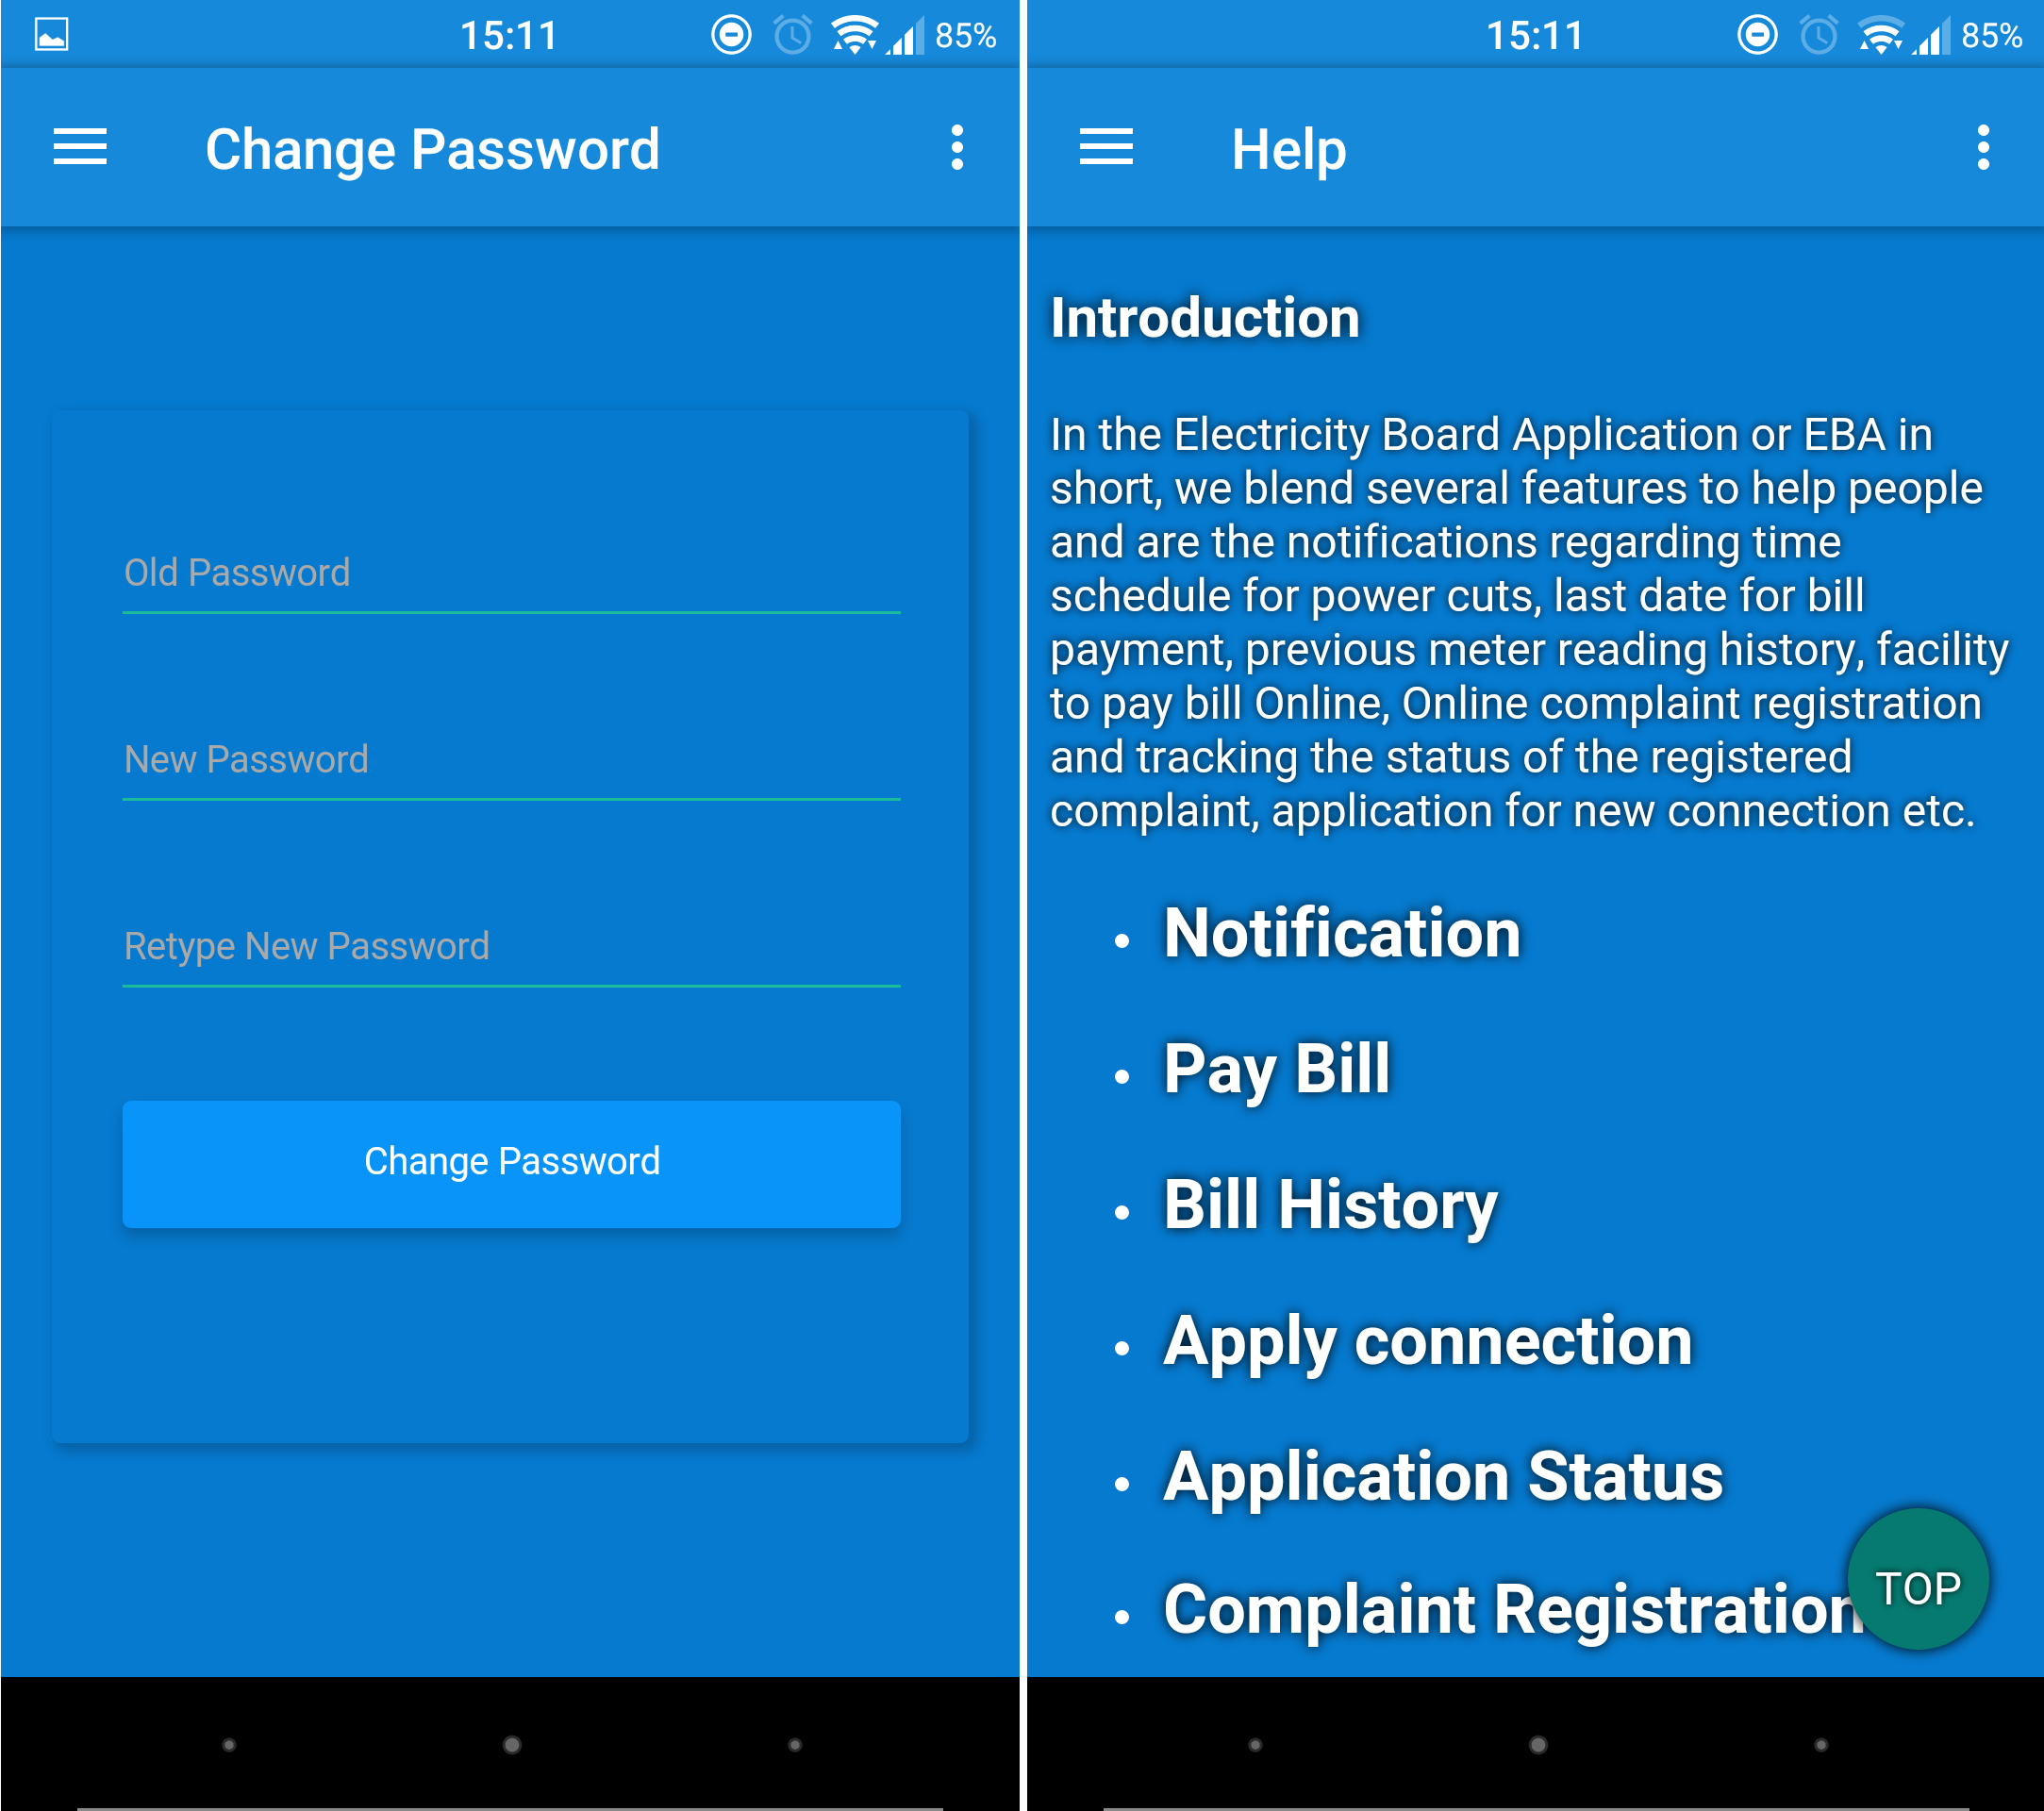
\includegraphics[width=11cm,height=10cm]{helppass.jpg}
			\caption{Change password and Help}
			\label{Change password and Help}
	\end{center}
\end{figure}
\textbf{Description}
\par Using the change password option we can update the password and by using help page user get the usage details about the application.

\newpage
\subsection{Home screen of Lineman}
\begin{figure}[h]
	\begin{center}
		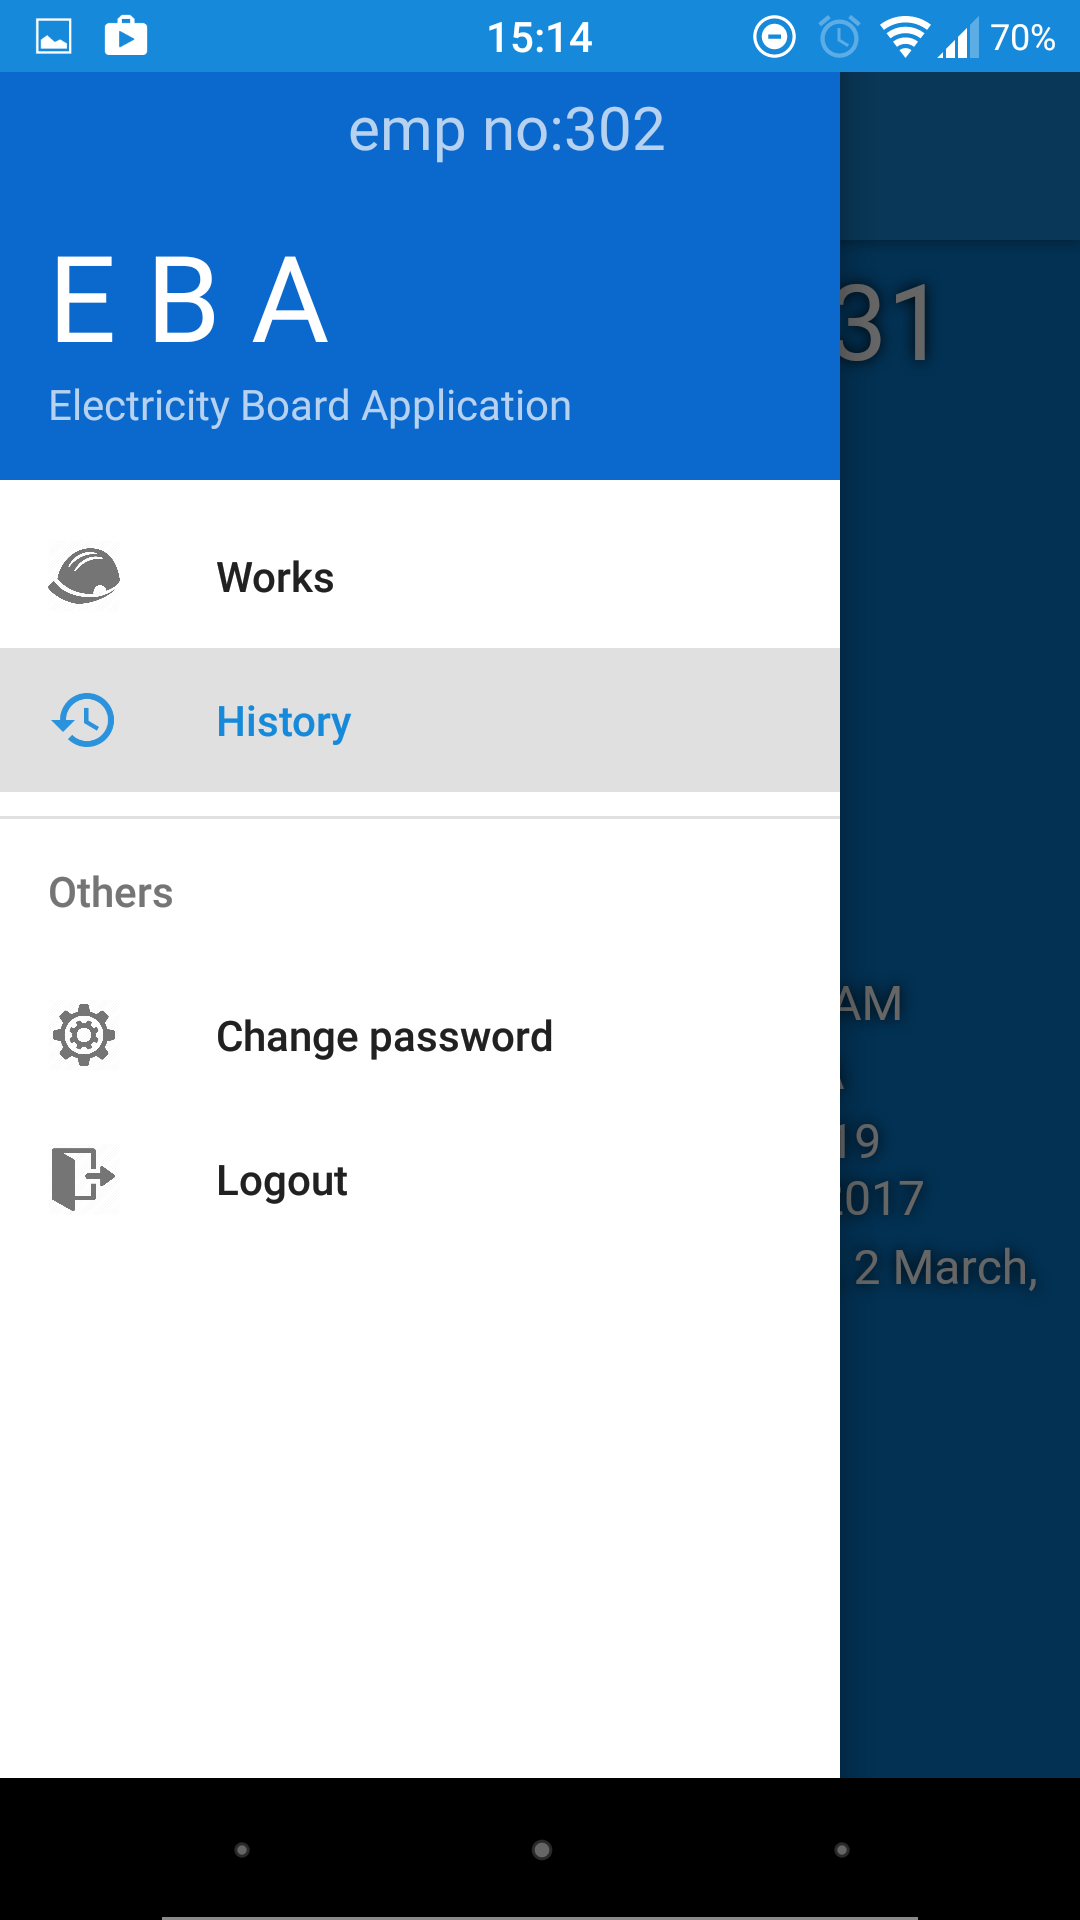
\includegraphics[width=7cm,height=12cm]{sslineman.png}
			\caption{Home screen of Lineman}
			\label{Home screen of Lineman}
	\end{center}
\end{figure}
\textbf{Description}
\par  This page has 3 choices. Those are work, history and change password.

\newpage
\subsection{Work and history}
\begin{figure}[h]
	\begin{center}
		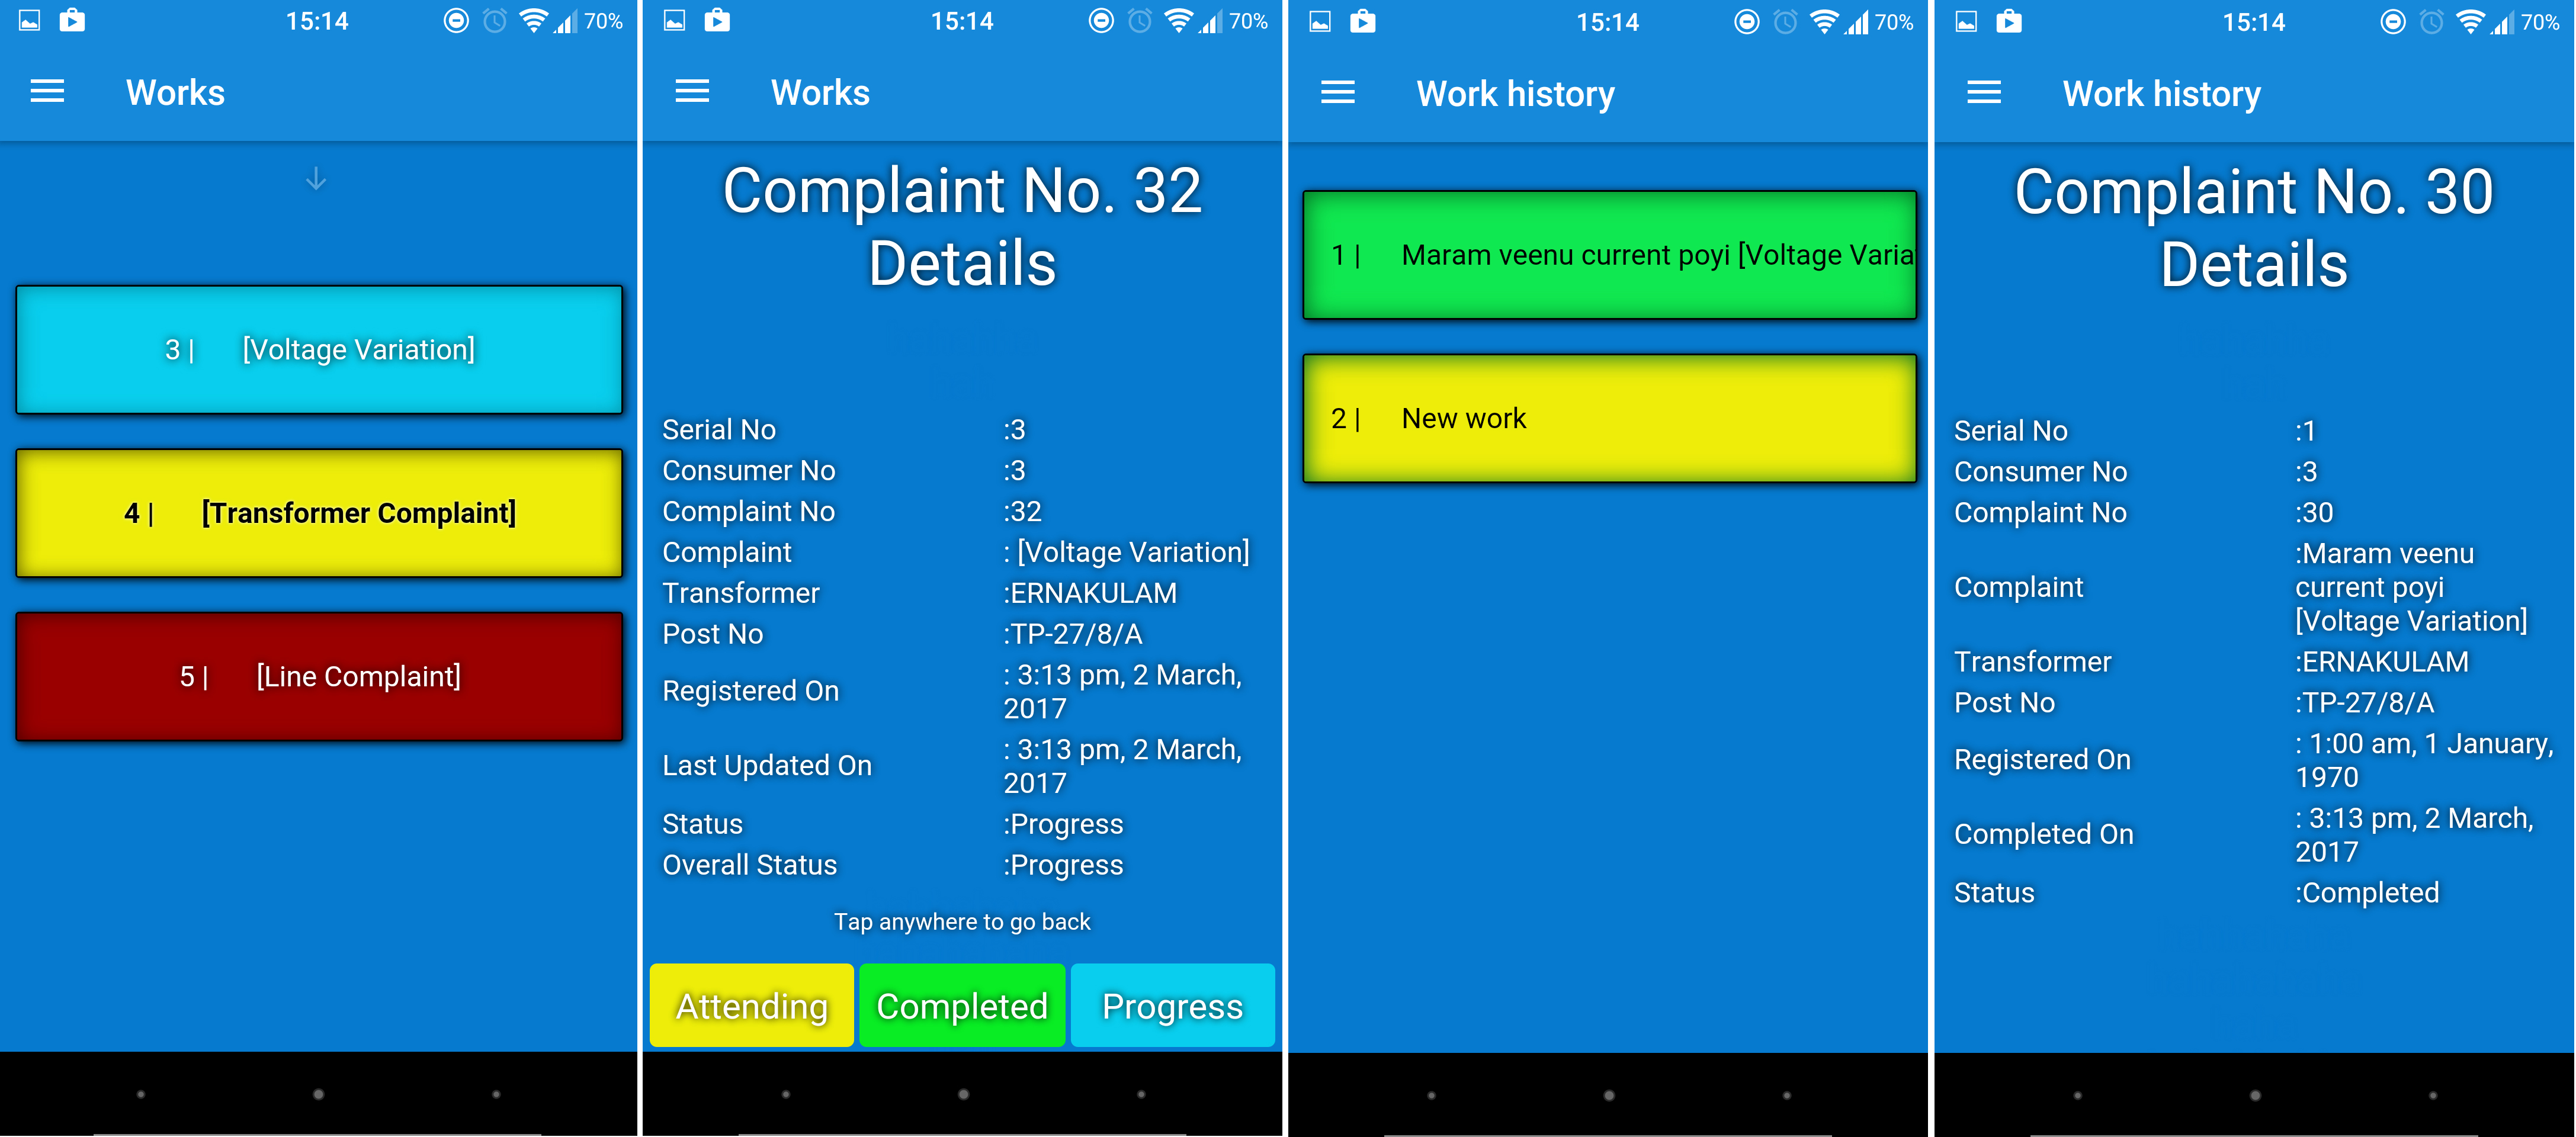
\includegraphics[scale=0.07]{linehome.jpg}
			\caption{Work and history}
			\label{Work and history}
	\end{center}
\end{figure}
\textbf{Description}
\par  Using work page lineman can view assigned tasks and view the history of works.

\newpage
\subsection{Administrator (system view)}
\begin{figure}[h]
	\begin{center}
		\includegraphics[width=15cm,height=9cm]{systemadmin.jpg}
			\caption{Admin side}
			\label{Admin side}
	\end{center}
\end{figure}
\textbf{Description}
\par  Administrator have the privilege over all users and can update database. 

\chapter{TESTING}
\par When a system is developed, it is hoped that it performs properly. In practice, however some errors always occur. The main purpose of testing an information system is to find the error and correct them. A successful test is one that finds an error. System testing is a critical aspect of Software Quality assurance and represents the ultimate review of specification, design and coding. Testing is the process of executing a program with the intent of finding an as yet undiscovered error. Nothing is complete without testing. Testing is vital to the success of the system.
\par The main objectives of the system testing are:
\begin{itemize}
\item To ensure during operation the system will perform as per specification.
\item To make sure that the system meets user requirements during operation.
\item To verify that the controls incorporated in the system function as intended.
 \end{itemize}
\par If the testing conducted successfully, it will uncover errors in the software. As a secondary benefit, testing demonstrates that the software functions appear to be working according to specification and that performance requirements appear to have been satisfied.
\par The system \quotes{EBA}is tested in such a way that almost all errors that may occur are found and corrected. The test process carried out in this system includes the following:
\section{CODE TESTING}
\par In code testing the logic of the developed system is tested. For this every module of the program is executed to find any error. To perform specification test, the examination of the specifications stating what the program should do and how it should perform under various conditions. This testing was done side by side with coding. This examines the logic of the program. In java special test cases are used for testing the code. Every part of the program was tested in this phase.
\section{PASSWORD TESTING}
\par This is done for user authentication. This process ensures security of the system thus avoiding unauthorized access to the system. When the user enters the username and password, checking it with the already registered usernames and passwords will validate him. If it matches then only the user is allowed to enter in to the system. Otherwise he is denied access and thereby strong security is provided. The password checking was done for the system. Only registered users were able to login.
\section{UNIT TESTING}
Unit testing is undertaken after a module has been coded and reviewed. Before carrying this testing, the unit test cases have to be designed and the test environment for the unit under test has to be developed. The various test cases are driver and stub modules. The main objective is to determine the correct working of the individual modules. During the testing each module is isolated from other modules and individually unit tested. It involves a precise definition of the test cases, testing criteria, and management of test cases. The modules that are tested include Client Terminal, Network Management and Server Management module.
 \section{INTEGRATION TESTING}
System testing does not test the software as a whole, but rather than integration of each module in the system. The primary concern is the compatibility of individual modules. One has to find areas where modules have been designed with different specifications of data lengths, type and data element name. Testing and validation are the most important steps after the implementation of the developed system. The system testing is performed to ensure that there are no errors in the implemented system. The software must be executed several times in order to find out the errors in the different modules of the system. Each of the modules were integrated together and subjected to testing.
\section{VALIDATION TESTING}
Validation refers to the process of using the new software for the developed system in a live environment i.e., new software inside the organization, in order to find out the errors. The validation phase reveals the failures and the bugs in the developed system. It will come to know of the practical difficulties the system faces when operated in the true environment. Validation test was performed in the Login section. By testing the code of the implemented software, the logic of the program can be examined. A specification test is performed to check whether the specifications stating the program are performing under various conditions. Apart from these tests, there are some special tests conducted which are given below:
\begin{itemize}
\item \textbf{Peak load test} This determines whether the new system will handle the volume of activities when the system is at the peak of its processing demand. The test has revealed that the new system is capable of handling the demands at the peak time.
\item \textbf{ Storage testing }  This determines the capacity of the new system to store transaction data on a disk or on other files. The proposed software has the required storage space available. 
\item \textbf{ Performance time testing } This test determines the length of the time used by the system to process transaction data.
 

\end{itemize}
 \section{SYSTEM TESTING}
 \par After all units of a program have been integrated together and tested system testing is taken up. It is same for both procedural and object oriented programming. System tests are designed to validate a fully developed system to assure that it meets its requirements. The system test cases can be classified into performance and functionality test cases. The functionality test cases are designed to check whether the software satisfies the functional requirements as documented in the SRS document. The performance tests on the other hand test the conformance of the system with non-functional requirements of the system.
 \section{OUTPUT TESTING}
 \par After the performance of unit testing, the next step is output testing. No system would be useful if it does not produce the required output in the specific format, thus output format on the screen is found to be correct when the format was designed in the system phase according to the user need.
 \par The maintenance of software is the time period in which software product performs useful works. Maintenance activities involve making enhancement to software product, adapting product to new environment and correcting problems. It includes both the improvement of the system function.  
\par It may involve the continuing involvement of a large proportion of computer department resources. The main task may be to adapt existing system in a changing environment. System should not be changed casually following informal requests. To avoid unauthorized amendments, all requests for change should be channelled to a person nominated by management. The nominated person has sufficient knowledge of the organization’s computer based systems to be able to judge the relevance of each proposed change. 
\par No annual costs for support or maintenance are required. Ofcourse, the individual system components come with limited warranty from the manufacturers, i.e., the PC, camera, etc. There is no obligation to purchase or pay for any extended maintenance or support.
\section{GOAL OF TESTING}
\par Many users may use our project. So the project designer must test all the modules of the project. The main goal of our project is, whenever user uses our project, it should run without any error.
\section{PASS/FAIL CRITERIA}
\par The pass/fail criteria specifies a set of constraints whose satisfaction leads to approval or disapproval of the proper functioning of the system .
\section{PASS CRITERIA}
\par The system must meet all the functional and non-functional requirements. Pass all the test cases, get the expected response, and get acceptable performance to be tested pass.
\begin{itemize}
\item User can login and choose various options.
\item  User can select facilities and the system will responds.
\item Periodic update of database
\end{itemize}
\section{FAIL CRITERIA}
\par If one of the following situations happens, the system is considered to fail:
\begin{itemize}
\item  User cannot login
\item  Database updation failure
\item  Human error
\end{itemize}


\newpage
\section{TEST REPORT}
\par The detailed test reports prepared for each function. A sample test report is given below:
\\
\begin{table}[!htb]
\centering
\caption{Test Report}
\label{Test Report}
\begin{tabular}{|l|l|}
\hline
Name                                                                                &  Electricity Board Application                                             \\ \hline
Version                                                                             & 1.0                                                                  \\ \hline
Author                                                                              & Muhammed Nadirsha, Ribin Roy, Ajesh M, Sreenivas s Naik         \\ \hline
Approved By                                                                         & Self                                                                 \\ \hline
Date                                                                                & Wednesday, 1st March 2017                                            \\ \hline
Role                                                                                & User can operate the system                                          \\ \hline
Prerequisite                                                                        & The user is logged into the system                                   \\ \hline
User/Actor                                                                          & System Response                                                      \\ \hline
Login                                                                               & User can enter their username and password to login.                 \\ \hline
Run Applications                                                                    & After successful authentication, the user can run those application. \\ \hline
Handle User Data                                                                    &                                                                      \\ \hline
                                                                                    &                                                                      \\ \hline
\begin{tabular}[c]{@{}l@{}}The test project\\ was successfully\\ saved\end{tabular} &                                                                      \\ \hline
\end{tabular}
\end{table}
\par Test case preparation helps the user and the developer to find and fix the errors easily and in advance. Berry Terminal is well tested with the proper test cases and thus passed a better unit test. Elaborated test cases also prepared subjected the system for thorough testing. The test cases prepared are in the following format.\\


\section{BLACKBOX TESTING}
\par Black-box testing is a method of software testing that examines the functionality of an application without peering into its internal structures or working. Test case preparation helps the user and the developer to find and fix the errors easily and in advance. Disease-Symptom Analyser using MapReduce is well tested with the proper test cases and thus passed a better unit test.\\
 The test cases prepared are in the following format:\\
 \\

\begin{table}[!htb]
\centering
\caption{Test Cases}
\label{Test Cases}
\begin{tabular}{|l|l|l|l|l|l|}
\hline
Test & Usecase step & \begin{tabular}[c]{@{}l@{}}Action performed\\ /User input\end{tabular} & \begin{tabular}[c]{@{}l@{}}Expected Result\\ /system response\end{tabular} & \begin{tabular}[c]{@{}l@{}}Actual          \\    result\end{tabular} & \begin{tabular}[c]{@{}l@{}}Do expected and \\ actual result cor-\\ respond\end{tabular} \\ \hline
1    & User         & \begin{tabular}[c]{@{}l@{}}Enter username \\ and password\end{tabular} & \begin{tabular}[c]{@{}l@{}}View sucess\\ page\end{tabular}                 & As Expected                                                          & Yes                                                                                     \\ \hline
2    & User         & Select option                                                             & \begin{tabular}[c]{@{}l@{}}View the \\ answer\end{tabular}                 & As Expected                                                          & Yes                                                                                     \\ \hline
3    & Application          & \begin{tabular}[c]{@{}l@{}}Replies to the \\ user\end{tabular}         & \begin{tabular}[c]{@{}l@{}}View the \\ answer\end{tabular}                 & As Expected                                                          & Yes                                                                                     \\ \hline
4    & User         & Logout                                                                 & \begin{tabular}[c]{@{}l@{}}View the login\\ page\end{tabular}              & As Expected                                                          & Yes                                                                                     \\ \hline
\end{tabular}
\end{table}


\chapter{FUTURE SCOPE}
\par In the proposed system all details about the system is designed into an application. It is designed as an android based application, which will work smoothly on any android phone except phones those having android version less than kitkat. For using the application, there will be no need of additional staff. Any person with basic android phone knowledge can use this application. Once the system is hosted on the network, the application will be automatically operated. Nowadays people are familiar with android and internet, and hence, they can easily use the options from the home page of the proposed application. So the proposed system is operationally feasible. Application is also supported by a powerful database where the data are arranged, making updates and collaboration easy and fast. The basic steps in application processing is same everywhere, and hence the extended version of this system be used in advanced areas too.  The existing system contain several problems . Currently the user suffering a lot with the existing system. There is a wastage of time and effort. The EBA is contain several facilities that will reduce the problems associated with the existing system. It reduces the burden of user who has to wait for the offline process in the existing system. The system will provide precise reply to the selected facility.




\chapter{CONCLUSION}
In the existing system people are suffering a lot because of the irregularities while interacting
with the electricity board. Proposed system is more user friendly. So user can easily
interact with the electricity board without any difficulties. In the Proposed system there are
number of features to help people to know about the information regarding time schedule for
power cuts, last date for bill payment, previous meter reading histories facility to pay bill
online and application for new connection. User will get informations about his/her current connection.
We know that the power cuts are more in the recent times and we are much irritated,
though the information about these power cuts are published in the dailies, people wont spot
the news efficiently, by using this application, people gets information about this data to their
application installed on the phone. so user can schedule their daily life programs according to
the informations. Also user can pay bill easily. There is another exciting option for user, that is,
user can pay their current bills through online. And also user can report their issues related to
current connection by online. Through which user will get efficient and fast service. Moreover,
all the services associated with the electricity board is collaborated into a single device.\\  
 


\newpage
\renewcommand{\bibname}{REFERENCES}
\begin{thebibliography}{999}
\addcontentsline{toc}{chapter}{\hspace{0.2in} REFERENCES}
	\bibitem{r1}Fundamentals of Software Engineering– Rajib Mall, Second edition, PHI, ISBN: 978-8-12-032445-
	9.
	\bibitem{r1}Software Engineering – Roger S. Pressman, Seventh illustrated edition, McGraw-Hill, ISBN: 978-0-
	07-337597-7.
  \bibitem{r1}IO Draw. \textit{http://www.draw.io.com/}
 \bibitem{r1}Tutorial point. \textit{http://www.tutorialspoint.com/}
  \bibitem{r1}w3schools.
  \textit{http://www.w3schools.com/}
   \bibitem{r1}Android developers.
    \textit{http:/developer.android.com/}
    \bibitem{r1}Youtube.
        \textit{http:/www.youtube.com/}
    \bibitem{r1}tizag.com.
        \textit{http:/www.tizaq.com/}
        \bibitem{r1}Github. \textit{http://www.github.com/}
        \bibitem{r1}stack overflow. \textit{http://www.Stackoverflow.com/}
        \bibitem{r1} Codeguru. \textit{http://www.codeguru.com/}
     
\end{thebibliography}

\addcontentsline{toc}{chapter}{\hspace{0.5cm}APPENDIX}
\chapter*{APPENDIX}
\appendix
\begin{lstlisting}

<?php
include('main.php');
$consumerno='';
$serial='';
    if(isset($_GET['serial'])){
        $serial=$_GET['serial'];
    }
$tempo='';
$erconsumerno='';
$ersectionno='';
$erphase='';
$erpostno='';
$ertransformer='';
$height=365;
     $connection = mysql_connect("localhost","root","nbuser");
     $db = mysql_select_db("eba", $connection);
     $query = mysql_query("SELECT * FROM `newconnection` WHERE
      `serialno` =$serial",$connection);
     $quer=mysql_fetch_assoc($query);
     $fieldempty=$quer['Status']; 
     mysql_close($connection);
?>
<html> 
<head>
<title>Verify Owner | EBA</title>
<link rel="stylesheet" href="stylew3.css">
<style>
    body {font-family: "Raleway", Arial, sans-serif;            
}
.noti input[type=text]:focus{
	outline: none;
	border: 1px solid rgba(255,255,255,0.9);
}
    .noti{
	position: absolute;
	top: 150px;
	left: 820px;
	height: 150px;
}
.noti input[type=submit]{
        float:right;
	width: 250px;
	height: 35px;
	font-weight: 400;
	padding: 6px;
}
    .noti input[type=text]{
	width: 250px;
	height: 35px;
	font-family: 'Exo', sans-serif;
	font-size: 16px;
	font-weight: 400;       
}
.noti input[type=text]{
	width: 250px;
	height: 35px;
        background-color:#f5f5f5;
	border: 1px solid
	font-size: 16px;
	font-weight: 400;        
}
.noti input[type=number]{
	width: 250px;
	height: 35px;
	font-family: 'Exo', sans-serif;
	font-size: 16px;
	font-weight: 400;
        }
.noti input[type=submit]:hover{
	opacity: 0.8;
}
.noti input[type=submit]:active{
	opacity: 0.6;
}
.noti input[type=submit]:focus{
	outline: none;
}
.parallax {
    background-image: url("main.jpg");
    background-attachment: fixed;
}
.w3-row img {margin-bottom: -8px}
</style>
</head>
<body>
    <div style="text-align:center;color:#FFFFFF;
    text-shadow: 0px 0px
     6px #000000;font-size:45px;">
        Verify Application 
    </div>
    
    <div style="width:1000px;padding-left:30px;">
    <div style="text-align:left;color:#FFFFFF;text-shadow:
     0px 0px
    6px #000000;font-size:22px;">
        <table> <tr><td>
        <table>
            <thead><tr><th>  </th><th></th></tr></thead>
            <tbody>
    <?php
    
    $billconnect = mysql_connect("localhost","root","nbuser");
    $db1 = mysql_select_db("eba", $billconnect);
    $ses_sql1=mysql_query("SELECT * FROM  `newconnection` 
    WHERE  `serialno` =$serial ", $billconnect);
    $rows = mysql_num_rows($ses_sql1);
    if (mysql_num_rows($ses_sql1) > 0) {
        while($row = mysql_fetch_assoc($ses_sql1)) {
        $consumerno=$row['appliedconsumerno'];
        echo "<tr><td>Name</td><td> : {$row[name]}</td></tr>";
        echo "<tr><td>Name of Organisation</td><td> : 
        {$row['organisation']}</td></tr>";
        echo "<tr><td>Name of authority</td><td> : 
        {$row['authorityname']}</td></tr>";
        echo "<tr><td>Category</td><td> : 
        {$row['category']}</td></tr>";
        $buildingno=$row['buildingnumber'];
        echo "<tr><td>Lane / Street</td><td> : 
        {$row['street']}</td></tr>";
        echo "<tr><td>Place / Landmark</td><td> : 
        {$row['place']}</td></tr>";
        echo "<tr><td>Pincode</td><td> : 
        {$row['pincode']}</td></tr>";
        echo "<tr><td>Village / Survey No</td><td> : 
        {$row['village']}</td></tr>";
        echo "<tr><td>Phone</td><td> : 
        {$row['phone']}</td></tr>";   
        echo "<tr><td>Name of Building</td><td> : 
        {$row['buildingname1']}</td></tr>";    
}
}
mysql_close($billconnect);
    ?> <?php
        if(isset($_POST['submit'])){
           // $tempo="inside isset";
            if ($_POST['submit']=='Update Status') {
                $category=$_POST['category'];
                $document='';
                if(isset($_POST['docs'])){
                    $document=$document." [".$count." 
                    ".$_POST['docs']."]";
                    $count++;
                }if(isset($_POST['docs1'])){
                    $document=$document." [".$count." 
                    ".$_POST['docs1']."]";
                    $count++;
                }if(isset($_POST['docs2'])){
                    $document=$document." [".$count." 
                    ".$_POST['docs2']."]";
                    $count++;
                }if(isset($_POST['docs3'])){
                    $document=$document." [".$count." 
                    ".$_POST['docs3']."]";
                    $count++;
                }if(isset($_POST['docs4'])){
                    $document=$document." [".$count." 
                    ".$_POST['docs4']."]";
                    $count++;
                }if(isset($_POST['docs5'])){
                    $document=$document." [".$count." 
                    ".$_POST['docs5']."]";
                    $count++;
                }if(isset($_POST['docs6'])){
                    $document=$document." [".$count." 
                    ".$_POST['docs6']."]";
                    $count++;
                }
                if($_POST['status']!=''){
                $status="Attention:".$_POST['status'];}
                $statusreport=$category;
                if($category=='Requesting Documents'){
                    $statusreport=$statusreport.":".$document;
                }
                $statusreport=$statusreport." ".$status;
                $billconnect = mysql_connect("localhost", 
                "root", 
                "nbuser");
                $db1 = mysql_select_db("eba", $billconnect);            
                $ses_sql1=mysql_query("UPDATE  
                `eba`.`newconnection`
                 SET  `Status` =  '$statusreport' WHERE  
                 `newconnection`.`serialno` ='$serial' ;", 
                 $billconnect);
                $notifi=mysql_query("INSERT INTO 
                `eba`.`notification` (`serialno`, `noti`, 
                `area`, `date`, `consumerno`) VALUES (NULL, 
                'Application Status Update for Building
                 Number : $buildingno | $statusreport', '0',
                  NOW(), '$consumerno');",$billconnect);           
                echo "<script>window.onload = function() {
                     if(!window.location.hash) {
                    window.location = window.location + 
                    '#loaded';
                    window.location.reload();
                    }
                    }</script>";
           $statusack="<font color=#00FF00>Status Updated
           </font>";
}
        if ($_POST['submit']=='Approve') {
            $consumerno='';
            $sectionno='';
            $postno='';
            $transformer='';
            $phase='';
            $tariff='';
            $billarea='';
            $csd='';
            $fixedcharge='';
            $meterrent='';
            $flag=0;
            if($_POST['consumerno']!=''){               
                $consumerno=$_POST['consumerno'];
            }
            else {
            $flag=1;                
                $erconsumerno="<font color=red> * </font>";
            }
            if( ! ctype_digit(strval($_POST['consumerno'])) 
            && $_POST['consumerno'] != '' ){
 $erconsumerno=$erconsumerno."<br><font color=red>
 <font size=2px>Consumer Number should be Integer</font>
 </font>";
 $flag=1;
 $height=$height+30;
}
            if( ! ctype_digit(strval($_POST['sectionno'])) 
            && $_POST['sectionno'] != '' ){
 $ersectionno=$ersectionno."<br><font color=red>
 <font size=2px>Section Number should be Integer</font>
 </font>";
 $flag=1;
 $height=$height+30;
}
            if($_POST['sectionno']!=''){
                $sectionno=$_POST['sectionno'];
            }else {
                $flag=1;
                $ersectionno="<font color=red> * </font>";
            }
            if($_POST['transformer']!=''){
                $transformer=$_POST['transformer'];
            }else {
                $flag=1;
                $ertransformer="<font color=red> * </font>";
            }
            if($_POST['postno']!=''){
                $postno=$_POST['postno'];
            }else {
                $flag=1;
                $erpostno="<font color=red> * </font>";
            }
            if($_POST['tariff']!=''){
                $tariff=$_POST['tariff'];
            }else {
                $flag=1;
                $ertariff="<font color=red> * </font>";
            }
            if($_POST['billarea']!=''){
                $billarea=$_POST['billarea'];
            }else {
                $flag=1;
                $erbillarea="<font color=red> * </font>";
            }
            if($_POST['csd']!=''){
                $csd=$_POST['csd'];
            }else {
                $flag=1;
                $ercsd="<font color=red> * </font>";
            }
            if($_POST['fixedcharge']!=''){
                $fixedcharge=$_POST['fixedcharge'];
            }else {
                $flag=1;
                $erfixedcharge="<font color=red> * </font>";
            }
            if($_POST['meterrent']!=''){
                $meterrent=$_POST['meterrent'];
            }else {
                $flag=1;
                $ermeterrent="<font color=red> * </font>";
            }
            if($_POST['phase']!=''){
                $phase=$_POST['phase'];
            }else {
                $flag=1;
                $erphase="<font color=red> * </font>";
            }
            if($flag==0){
            $billconnect = mysql_connect("localhost", "root", 
            "nbuser");
            $db1 = mysql_select_db("eba", $billconnect);
            $ses_sql1=mysql_query("SELECT * FROM 
             `newconnection` WHERE  `serialno` =$serial ", 
             $billconnect);
            $row = mysql_fetch_assoc($ses_sql1);
            $connection = mysql_connect("localhost", "root", 
            "nbuser");
            $db = mysql_select_db("eba", $connection);
            $search = mysql_query("SELECT *  FROM 
             `consumerdetails`  WHERE  `consumerno`
              =$consumerno");
            $rows = mysql_num_rows($search);
            $fieldempty="Consumer Number Already Registered 
            [".$consumerno."]";
            if ($rows == 0)
                {
                $ses_sql1=mysql_query("SELECT * FROM 
                 `newconnection` WHERE  `serialno` =$serial ", 
                 $billconnect);
                $row = mysql_fetch_assoc($ses_sql1);
                $ses_sql2=mysql_query("INSERT INTO 
                `eba`.`consumerdetails` (`serialno`, `name`, 
                `organisation`, `authorityname`, `category`, 
                `buildingname`, `buildingnumber`, `street`, 
                `place`, `pincode`, `village`, `phone`,
                 `buildingname1`, `buildingnumber1`, `street1` 
                 `place1`, `pincode1`, `village1`, 
                 `statusofapplicant`, `powerintensive`, 
                 `crossproperty`, `consentsobtained`, 
                 `supplypurpose`, `connectiontype`, `panno`, 
                 `aadhar`, `aconstruct`, `plotsize`,
                  `consumerno`, `sectionno`, `postno`,
                   `transformer`, `phase`, `tariff`,
                    `billarea`, `csd`, `fixedcharge`, 
                    `meterrent`,`registerdon`) VALUES (NULL, 
                    '{$row['name']}', '{$row['organisation']} 
                    '{$row['authorityname']}', 
                    '{$row['buildingname']}', 
                     '{$row['statusofapplicant']}', 
                    '{$row['powerintensive']}', 
                    '{$row['crossproperty']}', 
                    '{$row['consentsobtained']}', 
                    '{$row['supplypurpose']}', '$postno',
                     '$transformer',
                     '$phase', '$meterrent',NOW());", 
                     $billconnect);
                $ses_sql1=mysql_query("UPDATE  `eba`.
                `newconnection` SET  `Status` 
                =  'Approved' WHERE  `newconnection`
                .`serialno` ='$serial'
                 ;", $billconnect);
                $connectionbill = mysql_connect("localhost", 
                "root", "nbuser");
                $db = mysql_select_db("bill", $connectionbill);
                $ses_bill=mysql_query("CREATE TABLE  
                `b$consumerno` (
                `billno` INT( 150 ) NOT NULL AUTO_INCREMENT ,
                `billdate` DATETIME NOT NULL ,
                `pmrd` DATETIME NOT NULL ,
                `pbamount` FLOAT NOT NULL ,
                `ramount` FLOAT NOT NULL ,
                `creading` INT( 150 ) NOT NULL ,
                `preading` INT( 150 ) NOT NULL ,
                `consumption` INT( 150 ) NOT NULL ,
                `tamount` FLOAT NOT NULL ,
               PRIMARY KEY (  `billno` ) ,
               UNIQUE KEY  `billno` (  `billno` )
               ) ENGINE = INNODB DEFAULT CHARSET = latin1
               ;",$connectionbill);
            echo "<script>window.onload = function() {
                    if(!window.location.hash) {
                    window.location = window.location + 
                    '#loaded';
                    window.location.reload();   
                    }
                    }</script>";$fieldempty=
                    "Approved [".$consumerno."]";
            }
            if($rows>0) {
            }
            }
            else {
                $fieldempty="Field Empty";
            }
        }
        }
        ?>
        </table>
                </td><td>
        <form action="" method="post">
		<div class="noti" id="login">
                    <br>
                    <div id="statusbox" style="border: .5px 
                    solid black;border-radius:2px;
                    height:346px;padding:3px;">				
                                Status
   <select  name="category" style="width: 250px;
	font-weight: 400;">
  <option  value="Verification Under Progress">- Status 
  -</option>
  <option  value="Requesting Documents">Requesting Documents
  </option>
  <option  value="Waiting for Approval">Waiting for Approval
  </option>
  </select>
                   <br>              
<input type="checkbox" name="docs" value="Proof of Identity">
Proof of Identity<br>
<input type="checkbox" name="docs1" value="Letter of 
Authorisation">Letter of Authorisation<br>
<input type="checkbox" name="docs2" value="Details of Property 
Crossing & Consents">Details of Property Crossing & Consents
<input type="checkbox" name="docs3" value="Proof of ownership
">Proof of ownership<br>
<input type="checkbox"name="docs4" value="Consent from Owner">
Consent from Owner<br>
<input type="checkbox" name="docs5" value="Test Certificate of
 metering equipment">Test Certificate of metering equipment
<input type="checkbox" name="docs6" value="Agreement 
Dimensioned sketch">Agreement Dimensioned sketch<br>                                
<input type="text" placeholder="Explicit Status"name="status">
<br><br>                    
\right)   <?php echo "$statusack"; ?>
<input type="submit" style="background:orange;color:black;"
 name="submit" value="Update Status"><br>
                    </div>
<div id="approvalbox" style="border: .5px solid black;
border-radius:2px;height:750px;padding:3px;">
Consumer Number  <input type="number" placeholder="Consumer
 Number" name="consumerno"><br>
Section Number   <input type="number" placeholder="Section
 Number" name="sectionno"><?php echo $ersectionno ?><br><br>
Post Number   <input type="text" placeholder="Post Number"
 name="postno"><?php echo $erpostno ?><br><br>
Tariff  <input type="text" placeholder="Tariff" name=
"tariff"><?php echo $ertariff ?><br><br>
Bill Area  <input type="text" placeholder="Bill Area" name=
"billarea"><?php echo $erbillarea ?><br><br>
Meter Rent  <input type="number" placeholder="Meter Rent" 
name="meterrent"><?php echo $ermeterrent ?><br><br>
Phase <?php echo $erphase ?> <select  name="phase" style=
"width: 250px;
	height: 35px;
        background-color:#f5f5f5;
	border: 1px solid rgba(255,255,255,0.6);
	border-radius: 2px;
	color: #000;
        float:right;
	font-family: 'Exo', sans-serif;
	font-size: 16px;
	font-weight: 400;">
  <option  value="Single Phase">Single Phase</option>
  <option  value="Three Phase">Three Phase</option>
  </select><br><br>
  <?php echo $fieldempty; ?>
  <input type="submit" style="background:green;color:white;"
   name="submit" value="Approve"><br>               
                </div>
                </div> 
                </td>
            </tr>
        </table>
    </div>
    </div>
</html>       


    \end{lstlisting}


\chapter*{GLOSSARY}
\addcontentsline{toc}{chapter}{\hspace{0.2in} GLOSSARY}
\begin{itemize}
\item\textbf{ COCOMO}: Constructive Cost Estimation Model
\item\textbf{ DFD}: Data Flow Diagram
\item\textbf{ KLOC}: Kilo Lines Of Code
\item\textbf{ LOC}: Lines Of Code
\item\textbf{ HTML}: Hypertext Markup Language
\item\textbf{ GUI}: Graphical User Interface
\item\textbf{ OS}: Operating System
\item\textbf{ RAM}: Random Access Memory
\item\textbf{ UML}: Unified Modeling Language
\end{itemize}
\newpage
\addcontentsline{toc}{chapter}{\hspace{0.2in} INDEX}
\begin{theindex}
\hspace{.6in}\large B
\small
\item Blackbox Testing, 40\\
\hspace{.6in}\large C
\small
\item COCOMO, 8
\item Code Testing, 35
\item Cost Estimation, 8\\
\hspace{.6in}\large D
\small
\item Data Flow Diagram, 19, 20
\item Design, 11\\
\hspace{.6in}\large E
\small
\item Economical Feasibility, 6
\item Existing System, 3\\
\hspace{.6in}\large F
\small
\item Feasibility Study, 5
\item Features of Proposed System, 3 
\item Fail Criteria, 39
\item Future Scope, 42\\
\hspace{.6in}\large G
\small
\item Gantt Chart, 6
\item Goal of Testing, 39\\
\hspace{.6in}\large H 
\small
\item Hardware Requirements, 9\\
\hspace{.6in}\large I
\small
\item Integration Test, 37\\
\hspace{.6in}\large L
\small
\item Life Cycle Model, 4
\item Languages and Platform used, 24\\
\hspace{.6in}\large M
\small
\item Modules, 12\\
\hspace{.6in}\large N
\small
\item Non Functional Requirements, 37\\
\hspace{.6in}\large O
\small
\item Operational Feasibility, 6
 \item Output Testing, 37\\
\hspace{.6in}\large P
\small  
\item Pass Criteria, 39
\item Proposed System, 3
\item Purpose, 1
\item password Testing, 36 
\item Pass/Fail Testing, 39 \\
\hspace{.6in}\large R
\small
\item References, 45\\ 
\hspace{.6in}\large S
\small
\item Safety Requirements,10  
\item Screen shots, 26 
\item Scope, 1
\item Security, 6
\item Security Requirements, 10  
\item Sequence Diagram, 15 
\item Social Feasibility, 6
\item Software Requirements, 9 
\item System testing, 37
\item System Design, 11\\
\hspace{.6in}\large T
\small
\item Technical Feasibility, 6
\item Test Reports, 39\\
\hspace{.6in}\large U
\small
\item UML Diagram, 13
\item Use Case Diagram, 13
\item Unit Testing, 35\\
\hspace{.6in}\large V
\small
\item Validation Testing, 36\\
\end{theindex}
\end{document}
